

\section{Storyblok}
\setauthor{Peter Klose}

In Storyblok muss zuallererst die gewollte Struktur der Webseite widergespiegelt werden. Dies wird im Bereich 'Content' gemacht. 
Für Pfade mit Unterseiten werden Ordner erstellt und die restlichen Seiten  als 'Page', 'Branch' oder 'Article' definiert.
Die Content-Gestaltung und Festlegung findet dann in diesen 3 Typen statt. 


\subsection{Storyblok API}
Da Storyblok ein headless CMS ist, ist die einzige Möglichkeit auf die Daten zuzugreifen deren API-Schnittstelle im REST Standard. 
Die von Storyblok bereitgestellte API verwendet auch in Error Handling bekannte HTTP Error Meldungen. Wenn es keinen Fehler gibt, werden Daten im JSON Format weitergegeben. 
Die Basis URL des Endpoint lautet dabei wie folgt: \textbf{https://api.storyblok.com/v2}. Um jedoch die richtigen Daten zu erhalten müssen noch die 2 wichtigsten Parameter gesetzt werden, nämlich \textbf{version} entweder als \textbf{draft oder published} und der Token der zur Authentifizierung dient.
Sonstige Parameter beziehungsweise Einstellungen die verwendet wurden lauten:

\subsubsection*{Pagination}
Die Pagination ermöglicht es Listen von Elemten zu begrenzen, um sie dann mit mehreren Unterseiten verfügbar zu machen. Ein Beispiel wäre die News Seite. Sie lädt die neusten 25 News und wenn man auf 'weitere News' am Ende der Seite klickt erhält man die nächsten 25.
Hierfür werden die Parameter per\_page und page verwendet. Der standardmäßig eingestellte Wert für beide lautet 25 bei per\_page und 1 bei page.

\subsubsection*{Stories}
Stories stellen gesamte Seiten dar, wenn man also die \textbf{/ausbildung/it-medientechnik} URL aufrufen will, macht man, um alle Daten zu erhalten einen Request an die \textbf{https://api.storyblok.com/v2/cdn/stories/ausbildung/it-medientechnik} URL. 
Hiermit würde man einen Großteil der Daten bekommen jedoch nicht alle. Verlinkte News, die eine eigene URL besitzen, würde man nur als verlinke ID sehen. Um dieses Problem zu lösen, bietet Storyblok den sogenannten  \textbf{resolve\_relations} Parameter. Hinter diesen Parameter muss allerdings noch der richtige Verweis angegeben werden in folgenden Format: \textbf{component\_name.field\_name} somit werden dann wirklich alle Daten geladen, die benötigt werden, um die Seite darzustellen.

\subsection{Internationalisierung}
Storyblok bietet für die Internationalisierung 3 verschiedene Ansätze: Field Level translation, Folder Level translation und Space Level translation. 
In dieser Arbeit wurde der \textbf{Field Level Translation} Ansatz gewählt. 
Das Setup dafür schaut wie folgt aus:

Als Erstes müssen in den Einstellungen des Spaces unter dem Reiter 'Internationalization' die gewünschten Sprachen eingestellet werden. 
In diesem Fall war dies 'de' für Deutsch und 'en' für Englisch. 
Im Editor kann dann die Sprache auf Englisch gestellt werden und alle Felder, bei denen die Translation Checkbox angehakt ist, können übersetzt werden. 

Um diese Sprache dann auch auf der Webseite angezeigt zu bekommen, muss bei dem Request an die API am Ende einfach der Parameter \textbf{language=} angeben werden. 
In diesem Fall wäre dies \textbf{'de'} oder \textbf{'en'}.


\subsection{Bausteine der Webseite}
Wie der Name schon andeutet, handelt vieles in diesem headless CMS von Blöcken. Diese haben Variablen, welche dann im Editor mit Content befüllt werden können. 
Einen Überblick über alle verfügbaren Blöcke hat man in der Block library. Dort kann man auch neue Blöcke erstellen. In der finalen Version der Webseite sind 41 Blöcke zu finden. 

All unsere Blöcke enstprechen der selben Namensschreibweise. Dabei wird die Snake case Schreibweise verwendet, diese beginnen immer klein und mehrere Worte trennt ein \textunderscore  als Beispiel 'default\textunderscore component'.

In einem Block gibt es dann eine Ansammlung von Feldern, dabei gibt es mehrere zur Auswahl:

% https://www.storyblok.com/docs/schema-configuration#field-types

\begin{longtable}[c]{|l|p{10cm}|}
    \caption{Field Types, die von Storyblok bereitgestellt werden}
    \label{tab:beispiel} \\
    \hline
    \textbf{Feldname} & \textbf{Beschreibung} \\
    \hline
    \endhead
    %
    \hline
    \endfoot
    %
    Blocks & Weitere Blöcke können hinzugefügt werden. \\
    \hline
    Text & Einfaches einzeiliges Textfeld \\
    \hline
    Textarea & Mehrzeiliges Textfeld ohne Formatierung \\
    \hline
    Richtext & Mehrzeiliges Textfeld mit Formatierungsmöglichkeiten (JSON Format) \\
    \hline
    Markdown & Mehrzeiliges Textfeld mit Formatierungsmöglichkeiten (Markdown Format) \\
    \hline
    Number & Nummernfeld ohne Formatierung \\
    \hline
    Date/Time & Datum und Uhrzeit - Picker \\
    \hline
    Boolean & Checkbox - true/false \\
    \hline
    Multi-Options & Liste von Schlüssel-Wert-Paaren, die konfigurierbar sind. Entweder hartcodiert, als externes JSON oder als Datenbank. Mehrere Werte sind auswählbar \\
    \hline
    Single-Option & Liste von Schlüssel-Wert-Paaren, die konfigurierbar sind. Entweder hartcodiert, als externes JSON oder als Datenbank. Kein oder ein Werte sind auswählbar \\
    \hline
    Asset & Fileauswahl, die in den Typen limitiert werden kann (nur Images, Videos, Audio, Textdokumente) aber ansonsten alle Typen annimmt. \\
    \hline
    Multi-Assets & Fileauswahl, die in den Typen limitiert werden kann (nur Images, Videos, Audio, Textdokumente) aber ansonsten alle Typen annimmt. Mehrere Files können hier gleichzeitig ausgewählt werden. \\
    \hline
    Link & Link auf eine Unterseite aus Storyblok oder als externe URL \\
    \hline
    Table & In der größe Formatierbare Tabelle, keine Textformatierung möglich \\
    \hline
    Group & Gruppierungs Folder für die Attribute\\
    \hline
    Image(old) & Veraltete Option Bilder einzubinden - Asset sollte nun verwendet werden \\
    \hline
    File(old) & Veraltete Option Files einzubinden - Asset sollte nun verwendet werden \\
    \hline
    Plugin & Zugriff auf externe Storyblok-Pugins - UI UX differenziert mit jedem Plugin \\
    \hline
\end{longtable}

All diese Attribute haben ein Bearbeitungsfenster, welches von oben nach unten mindestens den Typen, Darstellungsnamen, Technischen Namen, Checkbox - Notwendig, Checkbox - Übersetzbar und Beschreibungsfeld bietet.

Die 2 Wichtigsten sind aber die beiden Checkboxen. Sie ermöglichen uns sicherzustellen, dass der Wert gesetzt werden muss (Checkbox - Notwendig) und dass man ihn falls Notwendig übersetzten kann (Checkbox - Übersetzbar). 

Nachstehen werden diese beiden Checkboxen mit den Spalten T für translateable und R für required dargestellt.

\subsubsection*{Page}
Der Page-Block war schon vorgefertigt von Storyblok und wurde genau so übernommen.
Dieser ist sehr simpel aufgebaut. Das einzige Attribut, welches er beinhaltet ist body, ein Blocks Element.

\subsubsection*{Article}
Article ist der Block, welcher für News, Projekte, Clubs bzw. Events benutzt wird. 
Wie Page ist er ein Root Level Block, er besitzt jedoch keinen dynamischen body sondern nur folgende Attribute

\begin{longtable}[c]{p{3cm}ccp{6cm}}
    \caption{Attribute des Article Blocks}
    \label{tab:article}\\
    \toprule
    \textbf{Attribute} & \textbf{R} & \textbf{T} & \textbf{Beschreibung} \\
    \midrule
    \endhead
    %
    \endfoot
    %
        headline & \checkmark & & Überschrift des Newsbeitrags oder Events \\
        subline & & \checkmark & Unterüberschrift \\
        type & \checkmark & & Typ des Artikels: News, Event, Projekt, Club \\
        allocate & & & Zugeordnete Abteilung, mitunter auch Allgemein, Sport oder Reisen \\
        date & \checkmark & & Erstellungsdatum, Datum des Events \\
        content & \checkmark & & Formatierter Text \\
        image & \checkmark & & Titelbild für diesen Beitrag \\
        assets & & & Weitere Medien \\
        subpage\_enabled & & & Soll ein Link zur vollen Seite dieses Beitrags angezeigt werden \\
\end{longtable}

\subsubsection*{Branch}
Branch spiegelt unsere Abteilungen wieder, er bietet wie Page einen body an Blocks und weitere wichtige Attribute zur richtigen Darstellung der Abteilungen sind:

\begin{longtable}[c]{p{3cm}ccp{6cm}}
    \caption{Attribute des Branch Blocks}
    \label{tab:article}\\
    \toprule
    \textbf{Attribute} & \textbf{R} & \textbf{T} & \textbf{Beschreibung} \\
    \midrule
    \endhead
    %
    \endfoot
    %
    headline & \checkmark & \checkmark & Abteilungsname \\
    subline & & \checkmark & Kurzbeschreibung der Abteilung \\
    allocate & & & Zugeordnete Abteilung \\
    imagevideo & & & Link zum YouTube-Video der Abteilung \\
    folder & & & Hinterlegter PDF-Folder der Abteilung \\
    description & & & Beschreibung der Abteilung \\
\end{longtable}

\subsubsection*{All Articles }
All Articles ist in Storyblok ein relativ simpler Block, er dient dazu alle Articles die zu einer bestimmten Kategorie gehören anzuzeigen.  

\begin{longtable}[c]{p{3cm}ccp{6cm}}
    \caption{Attribute des All Articles Blocks}
    \label{tab:article}\\
    \toprule
    \textbf{Attribute} & \textbf{R} & \textbf{T} & \textbf{Beschreibung} \\
    \midrule
    \endhead
    %
    \endfoot
    %
    headline & \checkmark & \checkmark & Überschrift \\
    type & \checkmark & & Article Kategorie Auswahl (News, Events, Projekte, Clubs) \\
    filter & & & Filtermöglichkeit der Articles (default: false) \\
\end{longtable}

\subsubsection*{Basic Slider}
Basic Slider ist wie der Name schon sagt ein einfacher Slider, welcher mit einem Mouse drag bedient wird. 
Da dieser Effekt aber nicht mehr in unser UI,UX-Design passt könnte es bei der Finalen Version dazu kommen, dass er durch den Scroll Slider ersetzt wird.

\begin{longtable}[c]{p{3cm}ccp{6cm}}
    \caption{Attribute des Basic Slider Blocks}
    \label{tab:blockname}\\
    \toprule
    \textbf{Attribute} & \textbf{R} & \textbf{T} & \textbf{Beschreibung} \\
    \midrule
    \endhead
    %
    \endfoot
    %
    headline & \checkmark & \checkmark & Überschrift \\
    content & \checkmark & & Mindestens 3 iFrame Container sind notwendig, andere Blocks sind nicht erlaubt \\
\end{longtable}

\subsubsection*{Classes}
Classes stellt die Struktur für die Darstellung der Klassen an der HTL dar. 
Es handelt sich um eine Abgeschlossene Sektion in seinem Content sind nur Class Entry Blocks erlaubt.

\begin{longtable}[c]{p{3cm}ccp{6cm}}
    \caption{Attribute des Classes Blocks}
    \label{tab:blockname}\\
    \toprule
    \textbf{Attribute} & \textbf{R} & \textbf{T} & \textbf{Beschreibung} \\
    \midrule
    \endhead
    %
    \endfoot
    %
    headline & \checkmark & \checkmark & Überschrift \\
    content & \checkmark & & Beliebige Anzahl von Class Entry Blocks \\
\end{longtable}

\subsubsection*{Classes Entry}
Classes Entry stellt wirklich genau eine Klasse dar. Gedacht wäre das Schul Klassenfoto als Repräsentation.  

\begin{longtable}[c]{p{3cm}ccp{6cm}}
    \caption{Attribute des Classes Entry Blocks}
    \label{tab:blockname}\\
    \toprule
    \textbf{Attribute} & \textbf{R} & \textbf{T} & \textbf{Beschreibung} \\
    \midrule
    \endhead
    %
    \endfoot
    %
    classname & \checkmark & & Name der Klasse \\
    img & \checkmark & & Klassenfoto der Klasse als Datei (nur Bilder erlaubt) \\
    headofclass & & & Klassenvorstand der Klasse \\
\end{longtable}

\subsubsection*{Custom Image}
Custom Image dient als Grundlage, wenn im Frontend spezielle Anforderungen an ein Bild gestellt sind. 
Als Beispiel die Broschüre in \emph{Über Uns}, diese musste gedreht werden.  

\begin{longtable}[c]{p{3cm}ccp{6cm}}
    \caption{Attribute des Custom Image Blocks}
    \label{tab:blockname}\\
    \toprule
    \textbf{Attribute} & \textbf{R} & \textbf{T} & \textbf{Beschreibung} \\
    \midrule
    \endhead
    %
    \endfoot
    %
    image & \checkmark & & Darzustellende Bilddatei \\
    type & & & Single-Select Liste der speziellen Anforderungen, wie es dargestellt werden soll \\
\end{longtable}

\subsubsection*{Custom Link}
Custom Link dient dazu alle Links die existieren gleich zu gestalten. Obwohl ein Link-Attribut in Storyblok existiert, haben wir uns nicht dafür ausgesprochen, weil es keine Möglichkeit gibt Symbole oder andere Spezielle Styles zu hinterlegen.  

\begin{longtable}[c]{p{3cm}ccp{6cm}}
    \caption{Attribute des Custom Link Blocks}
    \label{tab:blockname}\\
    \toprule
    \textbf{Attribute} & \textbf{R} & \textbf{T} & \textbf{Beschreibung} \\
    \midrule
    \endhead
    %
    \endfoot
    %
    link & \checkmark & & Link zu internen oder externen Medien bzw. Seiten \\
    symbol & & & Auswählbare Symbole, die vor dem Link angezeigt werden \\
    display\textunderscore name & \checkmark & \checkmark & Anzeigename des Links \\
\end{longtable}

\subsubsection*{Designable Table}
Storyblok bietet ein Plugin, welches es ermöglicht Tabellen darzustellen. Bei diesem Plugin ist es jedoch nicht möglich einen designten Body (fetter und farbiger Text) einzufügen. Aus diesem Grund wurde ein eigener Block erstellt, welcher diese Probleme beseitigt.

\begin{longtable}[c]{p{3cm}ccp{6cm}}
    \caption{Attribute des Designable Table Blocks}
    \label{tab:blockname}\\
    \toprule
    \textbf{Attribute} & \textbf{R} & \textbf{T} & \textbf{Beschreibung} \\
    \midrule
    \endhead
    %
    \endfoot
    %
    headline & & \checkmark & Überschrift \\
    columns & \checkmark & & Anzahl der gewünschten Spalten \\
    header & \checkmark & & Der 'Table Row' Block wird vorgesehen, die Menge ist dabei auf 1 limitiert \\
    body & \checkmark & $\geq 1$ & Mindestens ein 'Table Row' Block wird vorgesehen \\
\end{longtable}

\subsubsection*{Table Row}
Der Table Row Block, stellt eine Zeile der Tabelle dar. Aus diesem Grund wurde bei den Attributen des Blocks nur ein value hinterlegt, welches wieder ein 'Blocks' Element ist. Bei diesem ist die Blockauswahl auf 'Table Value' Limitiert.

\subsubsection*{Table Value}
Der 'Table Value' Block wurde so konfiguriert, sodass die einzige Eingabe ein Richtext-Element ist. Durch dieses wird eine komplette Formatierung gewährleistet.

\subsubsection*{Faq Collection}
Um die häufig gestellen Fragen und Antworten darstellen zu können, wurde eine FAQ Ansammlung erstellt.

\begin{longtable}[c]{p{3cm}ccp{6cm}}
    \caption{Attribute des Faq Collection Blocks}
    \label{tab:blockname}\\
    \toprule
    \textbf{Attribute} & \textbf{R} & \textbf{T} & \textbf{Beschreibung} \\
    \midrule
    \endhead
    %
    \endfoot
    %
    headline & \checkmark & \checkmark & Überschrift \\
    description & & & Zusätzliche Beschreibung als Richtext \\
    faqs & \checkmark & & Beliebige Anzahl von FAQ-Element Blocks \\
\end{longtable}

\subsubsection*{Faq Element}
Faq Element dient wiederum nur zur Befüllung der FAQ Collection.

\begin{longtable}[c]{p{3cm}ccp{6cm}}
    \caption{Attribute des Faq Element Blocks}
    \label{tab:blockname}\\
    \toprule
    \textbf{Attribute} & \textbf{R} & \textbf{T} & \textbf{Beschreibung} \\
    \midrule
    \endhead
    %
    \endfoot
    %
    question & \checkmark & \checkmark & Einfacher Text für die Frage \\
    answer & \checkmark & \checkmark & Richtext für eine formatierte Antwort \\
    video & & & Link zur Antwort-Video von Direktor DI Richard Kainerstorfer \\
    show\textunderscore video & & & Boolescher Wert ob das Video angezeigt werden soll oder nicht (default: false) \\
\end{longtable}

\subsubsection*{Footer}
Footer ist der Block, wie der Name schon sagt, der den Footer der Webseite widerspiegelt. Seine Attribute beinhalten nur footer\textunderscore bg - ein Bild welches zu speziellen Anlässen als Hintergrund verwendet werden kann und columns eine Ansammlung von Footer Col Blöcken.

\subsubsection*{Footer Col}
Der Footer Col Block ist eine Spalte des Footers - hierbei wurde eine Überschift der Spalte (headline) und eine Ansammlung an weiterführenden Links (links) für die Umsetzung eingerichtet.

\subsubsection*{Grid}
Der Grid Block wurde so eingerichtet, sodass alle gängigen Grids Konfiguriert werden können. Dafür wurden einige Attribute festgelegt.

\begin{longtable}[c]{p{3cm}ccp{6cm}}
    \caption{Attribute des Grid Blocks}
    \label{tab:blockname}\\
    \toprule
    \textbf{Attribute} & \textbf{R} & \textbf{T} & \textbf{Beschreibung} \\
    \midrule
    \endhead
    %
    \endfoot
    %
    content & \checkmark & & Ansammlung von Blöcken, die einen definierten oder konfigurierbaren Column Span haben \\
    columns & \checkmark & & Minimale Anzahl der Spalten \\
    mediumcolumns & & & Spaltenanzahl ab einer Breite von 768px \\
    largecolumns & & & Spaltenanzahl ab einer Breite von 1024px \\
    max\_w & & & Maximale Breite des Grids \\
    width & & & Definiert als Column Span (nur notwendig, wenn ein Grid in einem anderen Grid verwendet wird) \\
\end{longtable}

\subsubsection*{Grid Item}
Grid Item bietet den Content für das Grid, um vielseitig einsetzbar zu sein, sind viele Konfigurationen möglich.
\begin{longtable}[c]{p{3cm}ccp{6cm}}
    \caption{Attribute des Grid Item Blocks}
    \label{tab:blockname}\\
    \toprule
    \textbf{Attribute} & \textbf{R} & \textbf{T} & \textbf{Beschreibung} \\
    \midrule
    \endhead
    %
    \endfoot
    %
    headline & & \checkmark & Überschrift \\
    subline & & \checkmark & Unterüberschrift \\
    content & & \checkmark & Formatierbarer Text als Richtext \\
    width & & & Festlegung des Column Span des Elements \\
    type & & & Definiert den Stil des Elements (Ausbildung, Hochformat, Querformat) \\
    content\_type & & & Definiert, ob Main\_Image oder eine Animation angezeigt wird \\
    animation & & & Auswahl aus den verschiedenen Animationen der Abteilungen - nur verfügbar, wenn content\_type = animation \\
    main\_image & & & Hauptbild für dieses Grid-Item \\
    image\_right & & & Boolescher Wert (default: false) \\
    link & & & Link, auf den das gesamte Element verweist \\
    sub\_images & & & Ansammlung von mehreren zusätzlichen Bildern \\
    allocate & & & Zuordnung zu den Abteilungen \\
\end{longtable}

\subsubsection*{Headline}
Headline bietet die Möglichkeit, Blöcken ohne Überschrift oder Abschnitten eine passende Überschrift zu geben. Sie beinhaltet nur die Attribute headline und no\_spacing\_y.

\subsubsection*{Hero}
Hero definiert die oberste Sektion in all unseren Seiten - ausgenommen der Startseite. Die Besonderheit ist das schräge Bild und der zusätzlich mögliche Content.
\begin{longtable}[c]{p{3cm}ccp{6cm}}
    \caption{Attribute des Hero Blocks}
    \label{tab:hero}\\
    \toprule
    \textbf{Attribute} & \textbf{R} & \textbf{T} & \textbf{Beschreibung} \\
    \midrule
    \endhead
    %
    \endfoot
    %
    headline & \checkmark & \checkmark & Große Überschrift \\
    background\_image & \checkmark & & Bild, welches hinter der Überschrift liegt \\
    type & \checkmark & & Definiert das Aussehen des Hero Elements \\
    height & \checkmark & & Setzt die Höhe der Sektion \\
    fixed & & & Boolescher Wert, der die Position auf absolut setzt (default: false) \\
    hero\_features & \checkmark & & Blocks Attribut, das mit den Hero Feature Blöcken befüllt werden kann \\
    additional\_content & & & Wird nur bei News, Events und weiteren verwendet, der gesamte Inhalt befindet sich somit in der Hero Component \\
\end{longtable}

\subsubsection*{Hero Feature}
Zusätzliche Information kann hiermit neben dem Hero Block angezeigt werden. Dieser ist wieder konfigurierbar, um verschiedene Styles und Funktionen zu ermöglichen.
\begin{longtable}[c]{p{3cm}ccp{6cm}}
    \caption{Attribute des Hero Feature Blocks}
    \label{tab:blockname}\\
    \toprule
    \textbf{Attribute} & \textbf{R} & \textbf{T} & \textbf{Beschreibung} \\
    \midrule
    \endhead
    %
    \endfoot
    %
    symbol & & & Bietet eine Auswahl an Symbolen, die davor angezeigt werden können \\
    type & \checkmark & & Definiert die Darstellung entweder groß oder klein \\
    text & & & Dargestellter Text \\
    link & & & Falls notwendig, kann ein weiterführender Link angegeben werden \\
\end{longtable}

\subsubsection*{iFrame Container}
Um IFrames per Storyblok einbauen zu können, wurde der iFrame Container Block erstellt. Dieser bietet durch den Link die Möglichkeit beliebige IFrames wie Videos, Maps oder Ähnliches einzubinden. 
\begin{longtable}[c]{p{3cm}ccp{6cm}}
    \caption{Attribute des iFrame Container Blocks}
    \label{tab:blockname}\\
    \toprule
    \textbf{Attribute} & \textbf{R} & \textbf{T} & \textbf{Beschreibung} \\
    \midrule
    \endhead
    %
    \endfoot
    %
    headline & \checkmark & \checkmark & Überschrift \\
    iframe\_content & \checkmark & & Link zu dem einzubindenden iFrame \\
    links & & & Ansammlung von Custom Link Blocks \\
    additional\_info & & \checkmark & Formatierbarer Text als Richtext \\
\end{longtable}

\subsubsection*{Link Collection}
Ansammlung von Custom Link Blocks falls notwenig auch mit Überschift

\subsubsection*{Marquee}
Marquee Block bietet die Möglichkeit Content Horizonal automatisch scrollen zu lassen, so wie in einer Slideshow.
\begin{longtable}[c]{p{3cm}ccp{6cm}}
    \caption{Attribute des Marquee Blocks}
    \label{tab:blockname}\\
    \toprule
    \textbf{Attribute} & \textbf{R} & \textbf{T} & \textbf{Beschreibung} \\
    \midrule
    \endhead
    %
    \endfoot
    %
    content & $\geq 4$ &  & Ansammlung von Blöcken, die bewegt werden \\
    reverse\_direction & & & Dreht die Richtung der Marquee um (default: false) \\
    spacing\_top & & & Abstand oben (default: false) \\
    spacing\_bottom & & & Abstand unten (default: false) \\
    display\_all\_mobile & & & Wird der Marquee oder eine vertikale Liste angezeigt (nur auf Mobilgeräten, default: false) \\
    speed & & & Definiert die Geschwindigkeit der Marquee \\
\end{longtable}

\subsubsection*{Navbar}
So wie der Footer Block ist auch der Navbar Block die Implementierung der Navbar unserer Webseite.
\begin{longtable}[c]{p{3cm}ccp{6cm}}
    \caption{Attribute des Navbar Blocks}
    \label{tab:blockname}\\
    \toprule
    \textbf{Attribute} & \textbf{R} & \textbf{T} & \textbf{Beschreibung} \\
    \midrule
    \endhead
    %
    \endfoot
    %
    logo & \checkmark & & Logo, welches angezeigt wird \\
    logo\_dark & \checkmark & & Logo, welches im Darkmode angezeigt wird \\
    middle\_nav & & & Ansammlung von den hauptsächlichen Links \\
    side\_nav & & & Ansammlung von Links auf der rechten Seite \\
\end{longtable}

\subsubsection*{Scroll Slider}
Der Scroll Slider Block ist einer unserer Hauptfeatures. Durch ihn wird der horizontale Scroll in einen vertikalen Scroll umgewandelt.
\begin{longtable}[c]{p{3cm}ccp{6cm}}
    \caption{Attribute des Scroll Slider Blocks}
    \label{tab:blockname}\\
    \toprule
    \textbf{Attribute} & \textbf{R} & \textbf{T} & \textbf{Beschreibung} \\
    \midrule
    \endhead
    %
    \endfoot
    %
    title & \checkmark & \checkmark & Überschrift \\
    slider\_table & & & Tabelle, die zusätzliche Informationen anzeigen kann \\
    scroll\_start\_right & & & Festlegung, ob der Content der Start ist oder nichts \\
    slider & & & Blocks-Element zur Darstellung der Slider-Blöcke (nur Slider Item) \\
    alternating & & & Boolischer Wert, der festlegt, ob die Blöcke zentriert sind oder abwechselnd auf der Y-Höhe verschoben sind (default: false) \\
    scroll\_speed & & & Legt die virtuelle Höhe des Elements fest und somit die Schnelligkeit der seitlichen Verschiebung während des Scrollens \\
\end{longtable}

\subsubsection*{Scroll Slider Select}
Scroll Slider Select bietet die selbe Funktionalität wie der Scroll Slider, der Content wird aber nicht durch Blocks sondern durch das Auswählen beliebiger 'Article' Blocks festgelegt.
\begin{longtable}[c]{p{3cm}ccp{6cm}}
    \caption{Attribute des Scroll Slider Select Blocks}
    \label{tab:blockname}\\
    \toprule
    \textbf{Attribute} & \textbf{R} & \textbf{T} & \textbf{Beschreibung} \\
    \midrule
    \endhead
    %
    \endfoot
    %
    title & \checkmark & \checkmark & Überschrift \\
    show\_title\_animation & & & Soll die Startanimation (Logo-Schultransformation) abgespielt werden (default: false) \\
    scroll\_start\_right & & & Festlegung, ob der Content der Start ist oder nichts \\
    slider & & & Multi-Option zum Wählen der gewünschten Stories. Nur Stories mit dem Typen \emph{Article} werden akzeptiert \\
    scroll\_speed & & & Legt die virtuelle Höhe des Elements fest und somit die Schnelligkeit der seitlichen Verschiebung während des Scrollens \\
\end{longtable}

\subsubsection*{Site Jump}
Site Jump bietet die Möglichkeit zu verschiedenen Überschiften auf der selben Seite zu springen. Diese müssen als Jumplink in den Blocks Attribut 'headlines' angegeben werden und mit den zugeordneten headlines gleich sein. 

\subsubsection*{Slider Item}
Slider Item realisiert die einzelnen Contentbausteine von Scroll Slider.
\begin{longtable}[c]{p{3cm}ccp{6cm}}
    \caption{Attribute des Slider Item Blocks}
    \label{tab:blockname}\\
    \toprule
    \textbf{Attribute} & \textbf{R} & \textbf{T} & \textbf{Beschreibung} \\
    \midrule
    \endhead
    %
    \endfoot
    %
    headline & \checkmark & \checkmark & Überschrift \\
    subline & & \checkmark & Unterüberschrift \\
    content & & \checkmark & Formatierbarer Text als Richtext \\
    image & & & Hauptbild für dieses Element \\
    allocate & & & Zuordnung zu den Abteilungen \\
    type & \checkmark & & Definiert den Style des Elements (Event, Kontakt groß/klein, Bewerbung) \\
\end{longtable}

\subsubsection*{Spacer}
Der Spacer Block bietet die Möglichkeit falls notwendig mehr Platz zwischen 2 anderen Blöcken auf Y-Ebene einzufügen. Hierfür stehen folgende rem-Werte (2,4,6,8) im Size Attribut bereit.

\subsubsection*{Sponsor}
Der Sponsor Block wurde entwickelt, da die Sponsoren ein anderes Design benötigen, als es mit einem einfachen GridItem Block möglich ist. Die Besonderheit liegt im Ausblenden des zusätzlichen Contents.
\begin{longtable}[c]{p{3cm}ccp{6cm}}
    \caption{Attribute des Sponsor Blocks}
    \label{tab:sponsor}\\
    \toprule
    \textbf{Attribute} & \textbf{R} & \textbf{T} & \textbf{Beschreibung} \\
    \midrule
    \endhead
    %
    \endfoot
    %
    headline & & \checkmark & Name der Firma / des Sponsors \\
    subline & & \checkmark & Zusätzliche Info zum Sponsor \\
    image & \checkmark & & Logo des Sponsors \\
    link & & & Link zur gewünschten Adresse \\
    only\_image & & & Boolesche Auswahl, ob nur das Logo oder auch die headline und subline angezeigt werden sollen (default: false) \\
\end{longtable}


\subsubsection*{Table}
Wenn man einen relativ simplen Table benötigt ohne nennenswerte Textformatierung, dann bietet sich dieser Table Block an. Er beinhaltet nur den standardmäßigen Tabel, bereitgestellt von einem Storyblok Plugin.
\begin{longtable}[c]{p{3cm}ccp{6cm}}
    \caption{Attribute des Table Blocks}
    \label{tab:table}\\
    \toprule
    \textbf{Attribute} & \textbf{R} & \textbf{T} & \textbf{Beschreibung} \\
    \midrule
    \endhead
    %
    \endfoot
    %
    headline & & \checkmark & Überschrift über der Tabelle \\
    table & \checkmark & & Ein Table als Plugin wird verwendet, dieser kann dann nach Belieben bearbeitet und befüllt werden \\
\end{longtable}

\subsubsection*{Text}
Um textuellen Content wie in Datenschutz und auf dem Impressum mit Storyblok editierbar zu machen, wurde der Text Block implementiert. 
\begin{longtable}[c]{p{3cm}ccp{6cm}}
    \caption{Attribute des Text Blocks}
    \label{tab:blockname}\\
    \toprule
    \textbf{Attribute} & \textbf{R} & \textbf{T} & \textbf{Beschreibung} \\
    \midrule
    \endhead
    %
    \endfoot
    %
    headline & & \checkmark & Überschrift \\
    divider & & & Boolescher Wert, ob ein Divider zwischen headline und content angezeigt werden soll (default: false) \\
    content & & \checkmark & Formatierbarer Text als Richtext \\
    max\_w & \checkmark & & Legt die maximale Breite des Elements fest \\
\end{longtable}


\subsubsection*{Timetable}
Der Timetable Block bietet die Möglichkeit einen Stundenplan der HTL digital nachzustellen. Die Attribute sind headline und eine Ansammlung von Timetable Cols Blocks (columns).

\subsubsection*{Timetable Cols}
Die Timetable Cols spiegeln einen Tag im Stundenplan wieder. Sie beinhalten daher nur einen Text für den Tag (day) und eine Sammlung von Timetable Subject Blocks (subjects).

\subsubsection*{Timetable Subject}
Timetable Subject ist das Wichtigste und am meisten konfigurierbar am Timetable.
\begin{longtable}[c]{p{3cm}ccp{6cm}}
    \caption{Attribute des Timetable Subject Blocks}
    \label{tab:fach}\\
    \toprule
    \textbf{Attribute} & \textbf{R} & \textbf{T} & \textbf{Beschreibung} \\
    \midrule
    \endhead
    %
    \endfoot
    %
    name & \checkmark & & Name des Faches \\
    short\_name & \checkmark & & Kurzbezeichnung des Faches \\
    description & & \checkmark & Beschreibung des Faches \\
    is\_specialized\_subject & & & Legt fest, ob dieses Fach abteilungsspezifisch ist \\
    main\_image & \checkmark & & Bild, welches das Fach beschreibt \\
    color & & & Farbe des Faches, wie in Untis \\
    jahrgang1-5 & & & Nummerischer Wert, der die Stundenanzahl in den einzelnen Jahren beschreibt \\
\end{longtable}

\subsubsection*{Value Document}
Der Value Document Block ist für die Repräsentation des Wertedokuments an der HTL-Leonding. Es wurde ein eigener Block erstellt, um ein spezielles Design mit einer Schräge umsetzten zu können.
\begin{longtable}[c]{p{3cm}ccp{6cm}}
    \caption{Attribute des Value Document Blocks}
    \label{tab:dreieck}\\
    \toprule
    \textbf{Attribute} & \textbf{R} & \textbf{T} & \textbf{Beschreibung} \\
    \midrule
    \endhead
    %
    \endfoot
    %
    headline & & \checkmark & Überschrift \\
    subline & & \checkmark & Unterüberschrift \\
    content & & & Genau 5 Value\_document\_entry Blöcke werden vorausgesetzt \\
    background\_image & & & Hintergrundbild für das Dreieck auf der Seite \\
\end{longtable}

\subsubsection*{Value Document Entry}
Value Document Entry ermöglicht einen Eintrag in das Wertedokument. Die Attribute belaufen sich nur auf die Kernaussage des Wertes 'headline' und auf eine detailierte Beschreibung im Richtext-Format (description) 

\section{Next}
\setauthor{Peter Klose}

Am Start dieses Projekts war Next.js 13 die neuste Version und somit wurde dieses Projekt auch mit Next.js 13 in Verbindung mit dem neuen App Router erstellt.
Dies geschah durch den Befehl \emph{npx create-next-app@latest} dadurch war auch die gesamte Ordnerstruktur des Projekts fertig und die Template Seite konnte mit \emph{npm run dev} gestartet und auf \textbf{localhost:3000} aufgerufen werden.

\subsection{Struktur}
\subsubsection*{Folder}
Die von Storyblok generierten Folder sind \textbf{public} und \textbf{app}. 
Der public Ordner ist dabei für statische Assets verantwortlich. In unserer Implementierung wurde er nur für das Schullogo und eine Illustration der Schule verwendet. 
Der app Ordner ist aber der Wichtigste in dem ganzen Projekt. Er ist, wie schon vorher erwähnt, zuständig für das Routing der gesamten Webseite. 


Speziell von uns erstellt wurden die Ordner \textbf{animations}, \textbf{conponents}, \textbf{types} und \textbf{util} um eine bessere Übersicht über das Projekt zu erhalten. 
In den Ordnern befinden sich dann die dazugehörigen Dateien.

Unter \textbf{animations} sind dies alle exportierten Animation, die auf der Webseite angezeigt werden sollen, im JSON-Format. 

Unter \textbf{components} sind alle erstellen Components, wiederum aufgeteilt in Unterordner, um eine Struktur zu bewahren. Das wichtigste File in components ist aber der \textbf{StoryblokProvider.tsx}. Dieser ermöglicht die Verbindung zwischen Storyblok und Next.

Unter \textbf{types} ist das File \textbf{interface.tsx} zu finden. In diesem sind alle TS-Typen für das ganze Projekt festgehalten.

Unter \textbf{util} befinden sich dann noch 2 Files, welche rein technische TS Funktionen beinhalten.

\subsubsection*{Files}
Files im Root-Level des Projekts dienen hauptsächlich zur Konfiguration des Projekts. Dabei handelt es sich um die Files \textbf{.env.local}, \textbf{middleware.js}, \textbf{next-env.d.ts}, \textbf{next.config.js}, \textbf{package.json} und \textbf{tsconfig.json}.

Bei \textbf{.env.local} handelt es sich um das File, welches im lokalen Betrieb (npm run dev), die ganzen Konfigurationen beinhaltet. In unserem konkreten Fall sind dies nur der \textbf{STORYBLOK\_API\_KEY} und die \textbf{STORYBLOK\_API\_VERSION}.

In \textbf{middleware.js} wird eine Middleware ausgeführt, welche den Standort und im Zusammenhang damit die Sprache der Seite einstellt. Dafür wird am Start der URL ein /de oder ein /en eingefügt, falls nichts genannt und auch keine besonderen Optionen bekannt sind, wird standardmäßigen /de verwendet.

\textbf{next-env.d.ts} ist die TS Deklaration für Next.js

In \textbf{next.config.js} findet die Konfiguration des ganzen Projekt statt.

In \textbf{package.json} befinden sich die Abhängigkeiten und Skripte des Projekts.

\textbf{tsconfig.json} ist das Konfigurationsfile für TypeScript.

\subsection{Routing}
Um die Rute mywebsite.com/products/shoes/newest zu realisieren, müsste man im App Router (Ordner app) 3 Unterordner erstellen, sodass folgenden Ordnerstruktur entsteht app/products/shoes/newest. Bei statischen Seiten, wo der Content als HTML gepflegt wird, macht dies auch Sinn. All das, was man nachher auf der Webseite sehen will, muss in das 'page.tsx' File an der richtigen Stelle stehen. 
Da es sich aber bei Storyblok um dynamisch generierte Seiten handelt, bei denen man auch zusätzlich schon die Pfadstruktur anhand der Ordner und Seiten in Storyblok festlegt, wurde dieser Ansatz nicht geäht. Bei Änderungen der Struktur in Storyblok könnte es sein, dass die Seite gar nichtmehr funktioniert. 

Die Lösung dafür waren dynamische Routen realisiert durch Ordner, bei denen der Name in eckigen Klammern stand, ein sogenannter [Dynamic Segment] Ordner. Bei diesem Ordner handelt es sich um einen teilweise dynamischen Pfad. Er macht nämlich nur diese eine Stelle im Pfad dynamisch. Ein Beispiel dafür wäre app/blog/[slug]/page.tsx Pfade wie /blog/a /blog/b blog/b funktionieren alle, wenn man aber /blog/a/b eingibt ist dies nicht mehr möglich. 

Um dies zu ermöglichen, wurde ein Catch-all Statement verwendet. Dies ermöglicht ein Match aller weiteren Elemente. Dies wurde durch einen Ordner mit dem Namen [...slug] realisiert.

Die Ordnerstruktur des Projekt sieht also am Ende so aus /app/[lng]/[...slug]. Der [lng] Ordner wurde dabei absichtlich nicht in [...slug] inkludiert, damit alle Subpages einen eindeutigen Zugriff auf den lng Parameter haben. 
Um nun alle Seiten darstellen zu können, muss nur mehr die Page.tsx erstellt werden, welche im finalen Aufbau sehr simpel erscheint:

\begin{figure}[h]
    \centering
    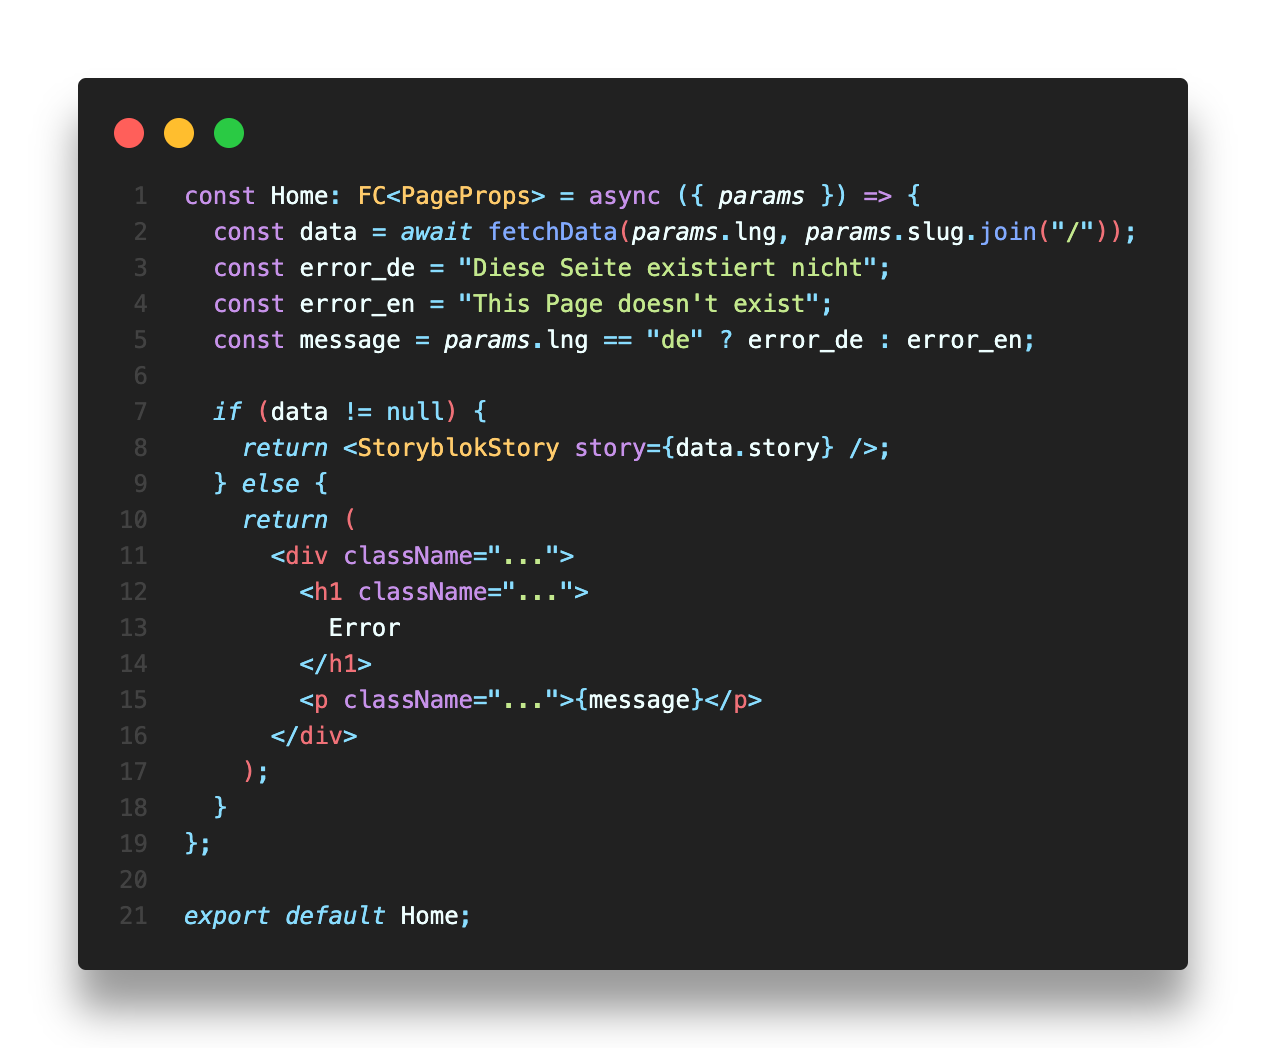
\includegraphics[width=\linewidth]{pics/final-page.png}
    \caption{Finales page.tsx}
    % \label{fig:impl:figma_entwurf}
\end{figure}

\subsection{Storyblok}
Nachdem die gerade erstelle Next13 Seite erfolgreich funktionierte, wurde das Storyblok Tutorial durchgearbeitet. Im späteren Verlauf der Arbeit stellten sich aber immer mehr Probleme im Bezug zu der am Anfang erstellten Verbindung festgestellen, sodass in der Mitte der Arbeit die Verbindung verändert wurde und am Schluss die komplette API-Schnittstelle selbst implementiert wurde.
Nicht nur das 5 Minuten Start Tutorial war noch nicht auf dem neuesten Stand sondern auch der Großteil der restlichen Tutorials, welche das Zusammenspiel von Next13 und Storyblok erklären sollte,  waren nicht auf den aktuellsten Stand beziehungsweise nicht auf den App Router Ansatz ausgelegt.

\subsubsection*{Verheiraten mit Next}
Nach mehreren Versuchen wurde dann der Storyblok Provider Ansatz gewählt. Dabei handelt es sich um ein Zusammenspiel einer Client Slide Component namens StoryblokProvider und dem Root Level layout.tsx file. Beide Files rufen dabei die storyblokInit() Funktion auf. 

Der StoryblokProvider übernimmt dabei die Aufgabe des Linkens der Components zu den Blocks von Storyblok.

\begin{figure}[H]
    \centering
    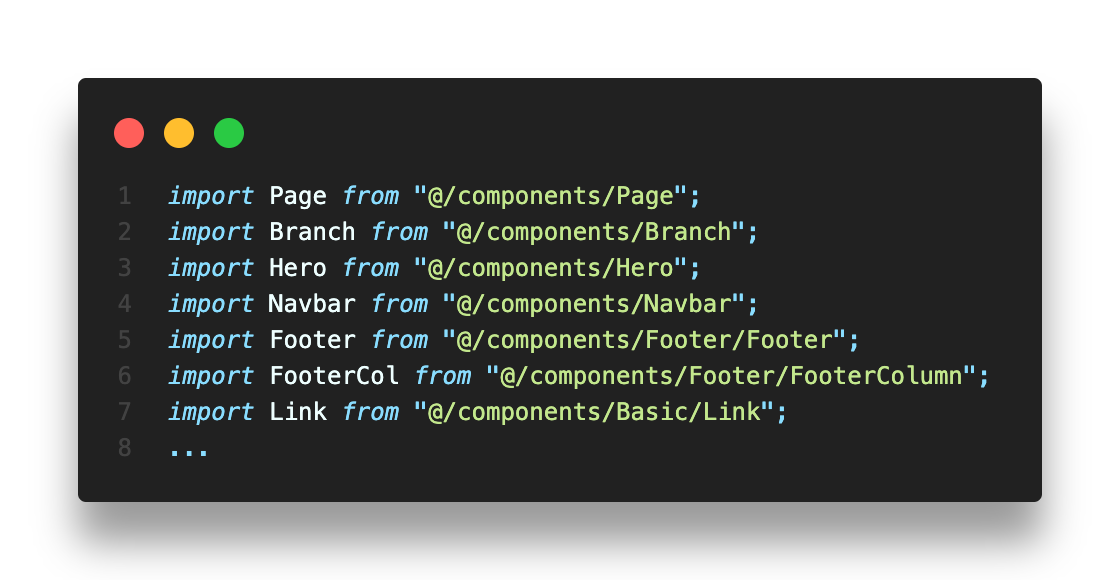
\includegraphics[width=\linewidth]{pics/sb-provider-01.png}
    \caption{Ausschnitt StoryblokProvider.tsx}
\end{figure}

Alle Componenten werden importiert und mit einem passenden Namen versehen. In einer Variable in diesem Fall \emph{const components} werden dann alle Storyblok Blöcke den Componenten zugeordnet.

\begin{figure}[H]
    \centering
    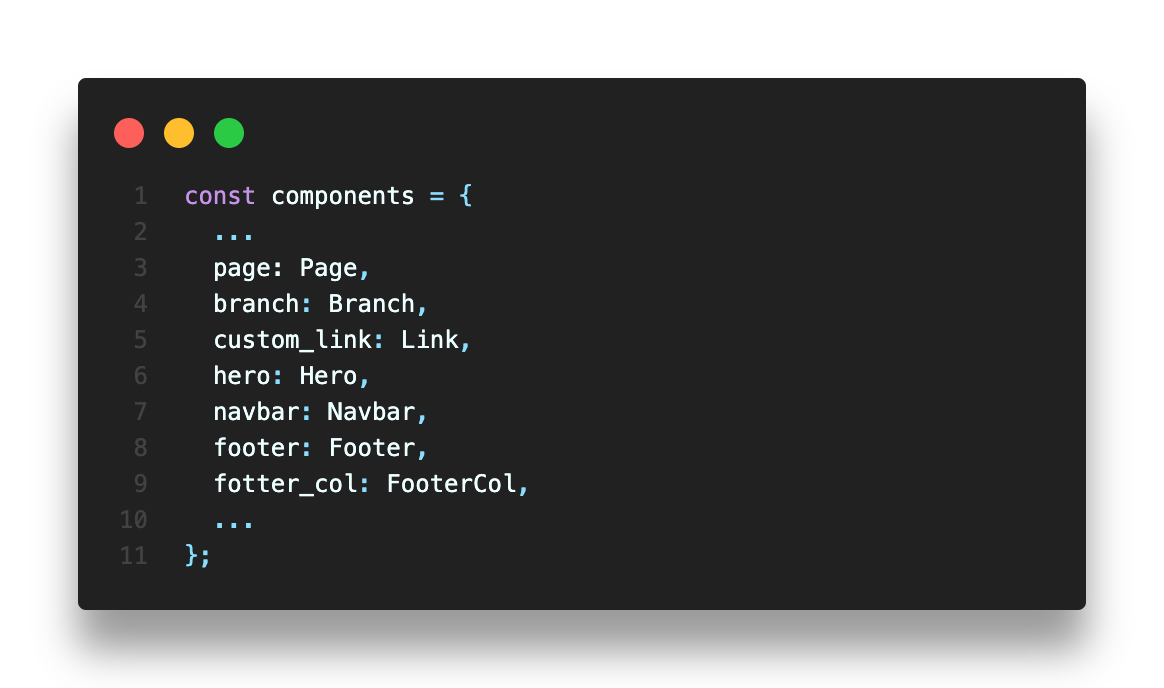
\includegraphics[width=\linewidth]{pics/sb-provider-02.png}
    \caption{Ausschnitt StoryblokProvider.tsx}
\end{figure}

Diese Ansammlung von Componenten kann dann in der storyblokInit Funktion mitgegeben werden, um Storyblok mit den Componenten zu verbinden. 

\begin{figure}[H]
    \centering
    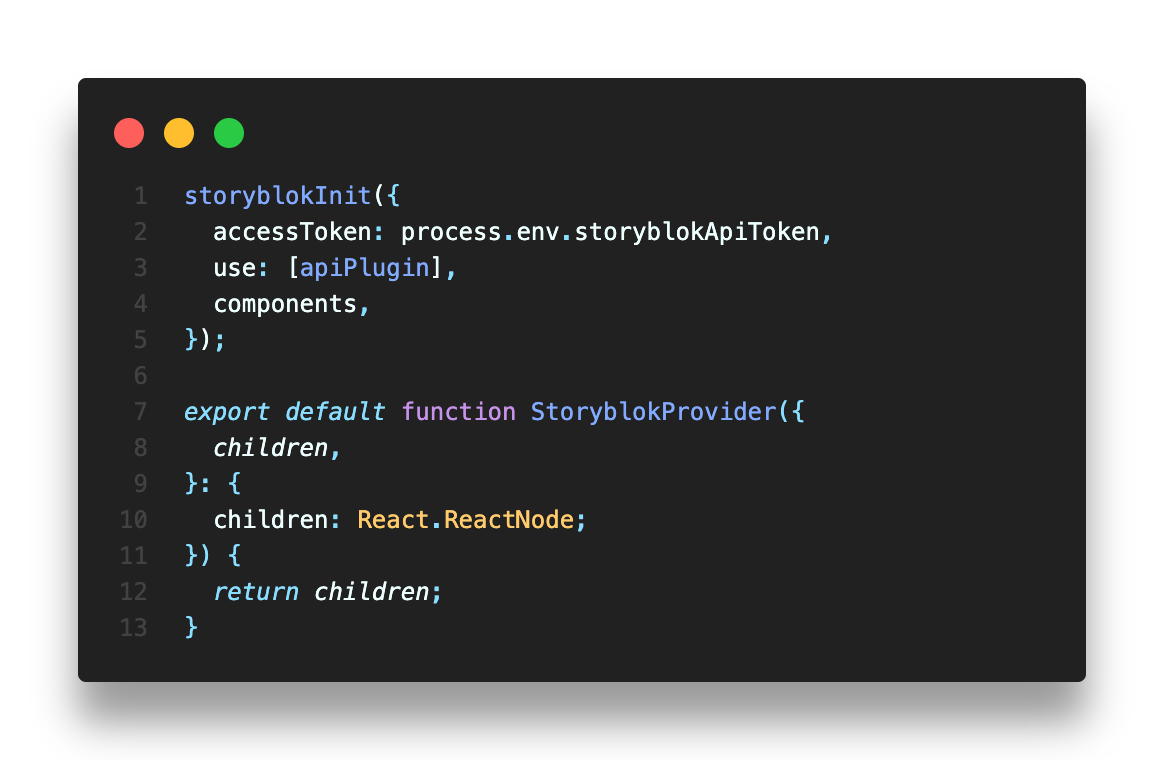
\includegraphics[width=\linewidth]{pics/sb-provider-03.png}
    \caption{Ausschnitt StoryblokProvider.tsx}
\end{figure}

\subsubsection*{Datenabfrage}
Da die von Stroyblok/react/rsc bereitgestellte storyblokApi.get() Funktion keine Next revalidation unterstützt, wurde der GET Request mittels JS fetch ausprogrammiert. 
Dabei trat das größte Problem bei den Sub-Stories auf. 
Sonst können diese durch die einfache Angabe der richtigen resolve\_relations Parameter gelöst werden. 
Wenn aber der API zugriff manuell erfolgt, befinden sich die 'Aufgelösten Beziehungen' ganz am Ende des JSONs und müssen manuell an die richtige Stelle transformiert werden. 

Dies wurde durch 2 Funktionen in einem Util File namens storyblok.tsx gelöst. 
Wobei die fetchData im Grunde genommen nur einen Fetch-Request an die API schickt und das Ergebnis dann im return an die weitere Funktion weitergibt.
\begin{figure}[H]
    \centering
    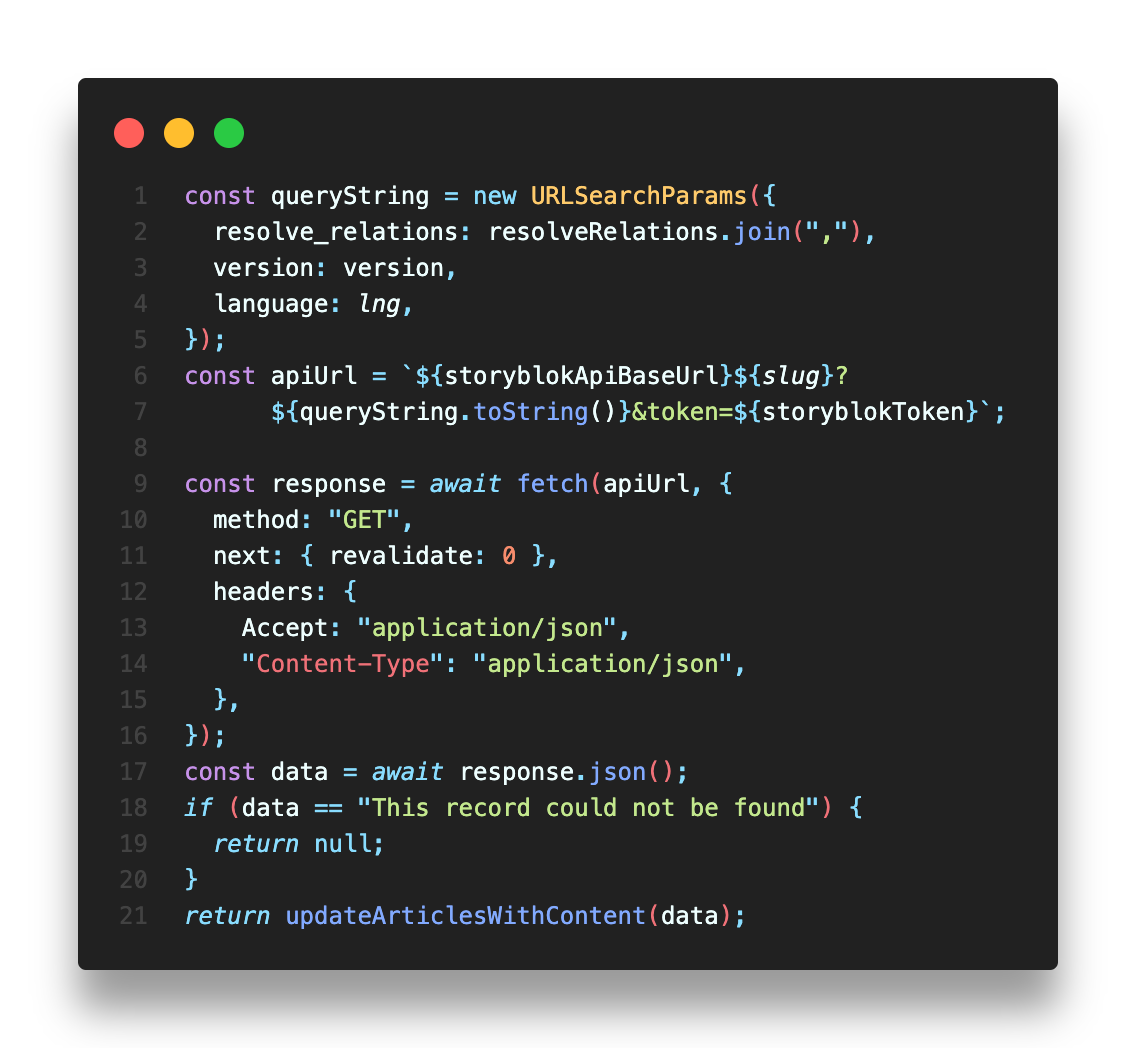
\includegraphics[width=\linewidth]{pics/sb-fetch-01.png}
    \caption{Fetch an Stroyblok-API}
\end{figure}

Die andere Funktion, welche man am Ende dieses Codeausschnitts sehen kann, ist aber von weitaus größerer Bedeutung. Sie löst das vorhin angesprochene Problem der 'resolve Relations'. Sie speichert alle Verweise und die dazugehörigen originalen Daten. Folgend werden alle Elemente in der Story überprüft, ob sie den passenden UUID beinhalten. Wenn ja, wird der Content ausgetauscht. Diese Erklärung entspricht nicht ganz der Realität, da in der Realität Zwischenabfragen die Performance erhöhen somit wird nur die UUID verglichen, wenn es sich um das Attribut atricles oder slider handelt.
\begin{figure}[H]
    \centering
    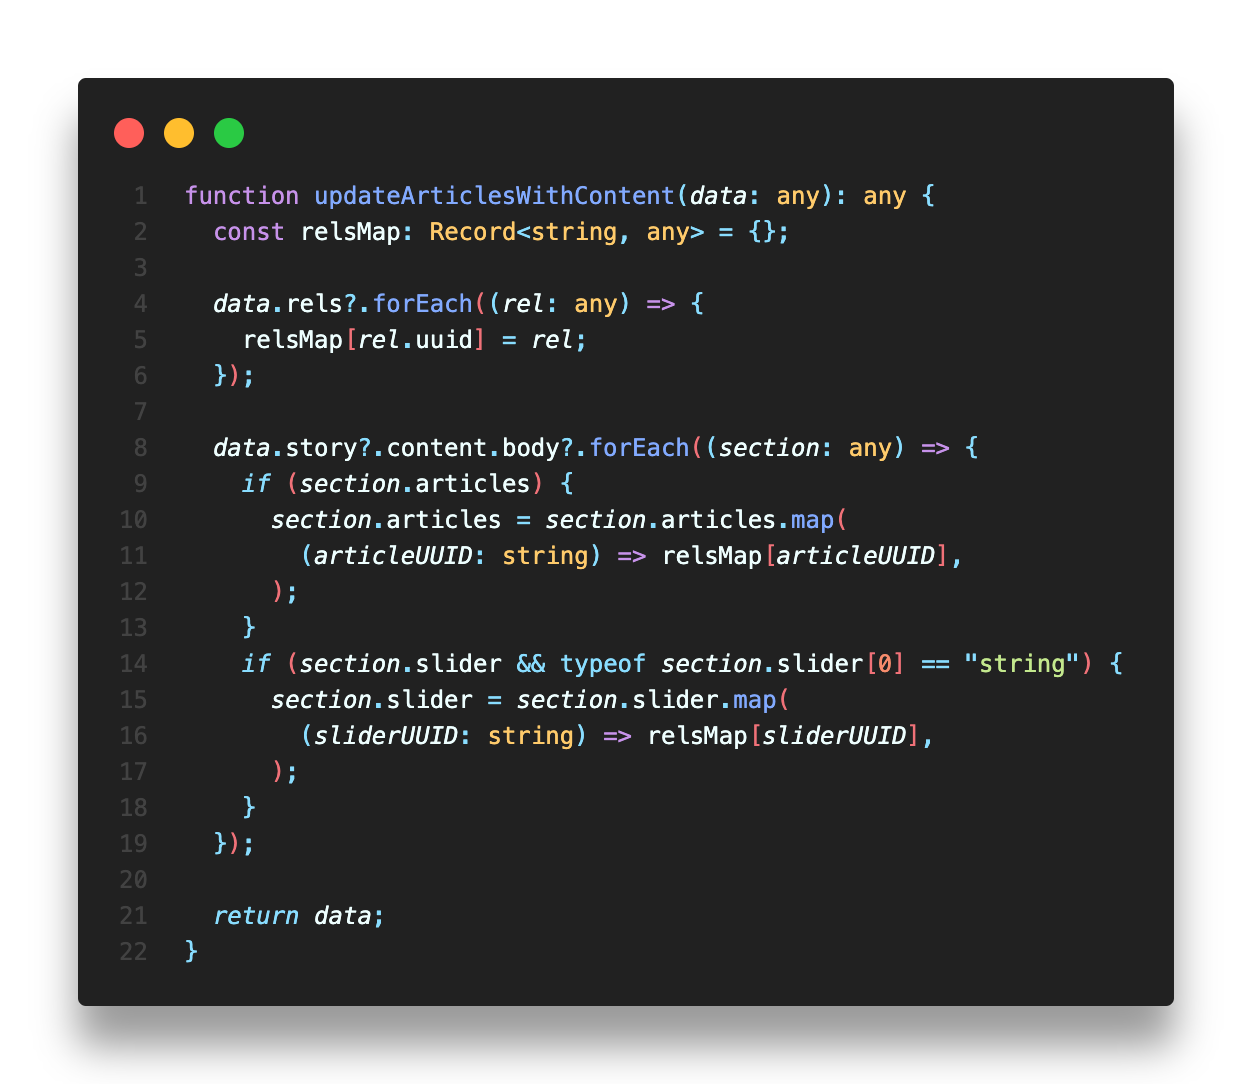
\includegraphics[width=\linewidth]{pics/sb-fetch-02.png}
    \caption{Datentransformation - Storyblok Fetch}
\end{figure}


\subsection{Packages}
Da es sich bei diesem Projekt um eine Node basierte Architektur handelt, wurden einige Packages als Erweiterungen installiert. 
Packages, welche in Kombination mit Storyblok stehen, werden hier nicht angeführt und werden in den Unterkapitel Storyblok näher beschrieben werden. Auch Packages wie react und typescript werden hier nicht behandelt, da sie nicht explizit hinzugefügt worden sind und somit die Basis des Projektes bilden.

\subsubsection*{Framer Motion}
Framer Motion ist eine Animationsbibliothek für React. In dieser Diplomarbeit übernimmt Framer Motion alle Animationen mit Ausnahme von den SVG Animationen. Diese werden von React-Lottie abgespielt.

Bevor man Framer Motion verwenden kann muss man es installieren, da es ein Node-Package ist, ist dies nicht schwierig: \emph{npm install framer-motion}.

Die Verwendung von Framer Motion ist simpel. Überall dort wo es verwendet werden soll muss man es importieren: \emph{import \{ motion \} from "framer-motion"}.
Wenn man also nun aus einem html Tag ein Motion html Tag machen will, muss man vor den Tag ein \textbf{motion.} schreiben als Beispiel ein \textless div\textgreater wird zu einem \textless motion.div\textgreater.   



\subsubsection*{TailwindCss}
Tailwind CSS ist ein modernes Utility-First-CSS-Framework für das Erstellen von benutzerdefinierten und skalierbaren Designs. Mit einer umfangreichen Sammlung von vorgefertigten Utility-Klassen können schnell und einfach flexible Layouts und ansprechende Benutzeroberflächen erstellt werden. Durch die Verwendung von Tailwind CSS kann der HTML-Code vereinfacht und gleichzeitig die Flexibilität bewahrt werden, um maßgeschneiderte Designs zu erstellen. 

Die Installation von Tailwind CSS ist unkompliziert über npm möglich: \emph{npm install tailwindcss}. Nach der Installation kann Tailwind CSS einfach in das Projekt integriert und in HTML-Dateien verwendet werden.

\subsubsection*{React Lottie}
React Lottie ist eine React-Komponente, die die Integration von animierten Lottie-Dateien in React-Anwendungen ermöglicht. Lottie ist ein von Airbnb entwickeltes Tool, das es Designern ermöglicht, komplexe Animationen zu erstellen und sie als JSON-Dateien zu exportieren. Diese JSON-Dateien können dann mit React Lottie in React-Anwendungen eingebettet und abgespielt werden. 

Mit React Lottie können Entwickler ansprechende Animationen in ihre Anwendungen integrieren, um die Benutzererfahrung zu verbessern. Die Installation von React Lottie erfolgt über npm: \emph{npm install react-lottie}.

\subsubsection*{React Icons}
React Icons ist eine Sammlung von vorgefertigten Icons, die als React-Komponenten bereitgestellt werden. Diese Icons können einfach in React-Anwendungen eingebettet und angepasst werden, um eine ansprechende Benutzeroberfläche zu erstellen. React Icons bietet eine Vielzahl von Symbolen und Symbolbibliotheken, darunter Font Awesome, Material Icons und mehr. 

Die Integration von React Icons in ein Projekt erfordert lediglich die Installation des Pakets über npm: \emph{npm install react-icons}.

\subsubsection*{React Fast Marquee}
React Fast Marquee ist eine React-Komponente, die das einfache Hinzufügen von horizontalen Scrollanimationen zu Elementen ermöglicht. Diese Komponente eignet sich ideal für das Erstellen von animierten Laufbändern, Bildergalerien und anderen interaktiven Elementen, die horizontal scrollen. React Fast Marquee bietet eine schnelle und effiziente Möglichkeit, Scrollanimationen zu implementieren, ohne aufwändige Konfigurationen oder zusätzliche Abhängigkeiten. 

Die Installation von React Fast Marquee erfolgt über npm: \emph{npm install react-fast-marquee}.

\subsection{Komponenten}

Für fast jeden Block im Storyblok-Backend wurde in Next eine Komponente erstellt. Die Daten werden dann mithilfe von TypeScript typisiert übergeben und können so richtig dargestellt werden. Da die meisten Komponenten sehr logisch strukturiert und aufgebaut sind, wird hier nicht mehr weiter darauf eingegangen. Die folgenden Komponenten die dennoch beschrieben werden, weichen von den vorher angemerkten Eigenschaften ab, da sie spezielle Berechnungen beinhalten, eine andere Datenstruktur aufweisen und die Hauptaugenmerke unserer Webseite darbieten.

\subsubsection*{ScollSlider und ScrollSliderSelect}

Die wichtigste und auffälligste Komponente ist dabei der ScrollSlider, insbesondere der ScrollSlider mit den Funktionen Select oder Latest. Diese Kombination bietet die Möglichkeit, den Bildlauf von der Y-Achse zur X-Achse zu transformieren. Dadurch scrollt der Benutzer nicht mehr wie gewohnt von oben nach unten, sondern von links nach rechts. Auf diese Weise wird der Fokus des Benutzers auf den angezeigten Inhalt gelenkt, da der normale Fluss der Webseite unterbrochen wird.

Der ScrollSlider lässt sich in drei Varianten unterteilen: Select, News und Custom.

Beim Select ScrollSlider können beliebige Blöcke, die den Typen Article besitzen, ausgewählt und angezeigt werden.
Beim News-Slider wird der Select ScrollSlider so umfunktioniert, dass automatisch die letzten x Neuigkeiten geladen werden; standardmäßig sind dies 5 Stück.
Die Custom-Variante des ScrollSliders enthält eine beliebige Anzahl von SliderItems, die mit unterschiedlichstem Inhalt gefüllt sein können.

Die technische Realisierung wurde so gestaltet, dass die Bildschirmbreite des Fensters ermittelt wird und der Inhalt dann am Anfang des Fensters platziert wird. 
Darüber hinaus ist von jedem Element im Slider die Breite bekannt, sodass die virtuelle Breite optimal ausgenutzt werden kann. 
Die Grundlage dafür bildete ein YouTube-Tutorial mit dem Titel \emph{Horizontal Scrolling Animation with React and Framer Motion} von \emph{Tom Is Loading}. Link: \emph{https://www.youtube.com/watch?v=4ehYkfh7P-I}. 

\begin{figure}[H]
    \begin{minipage}[b]{.4\linewidth} 
        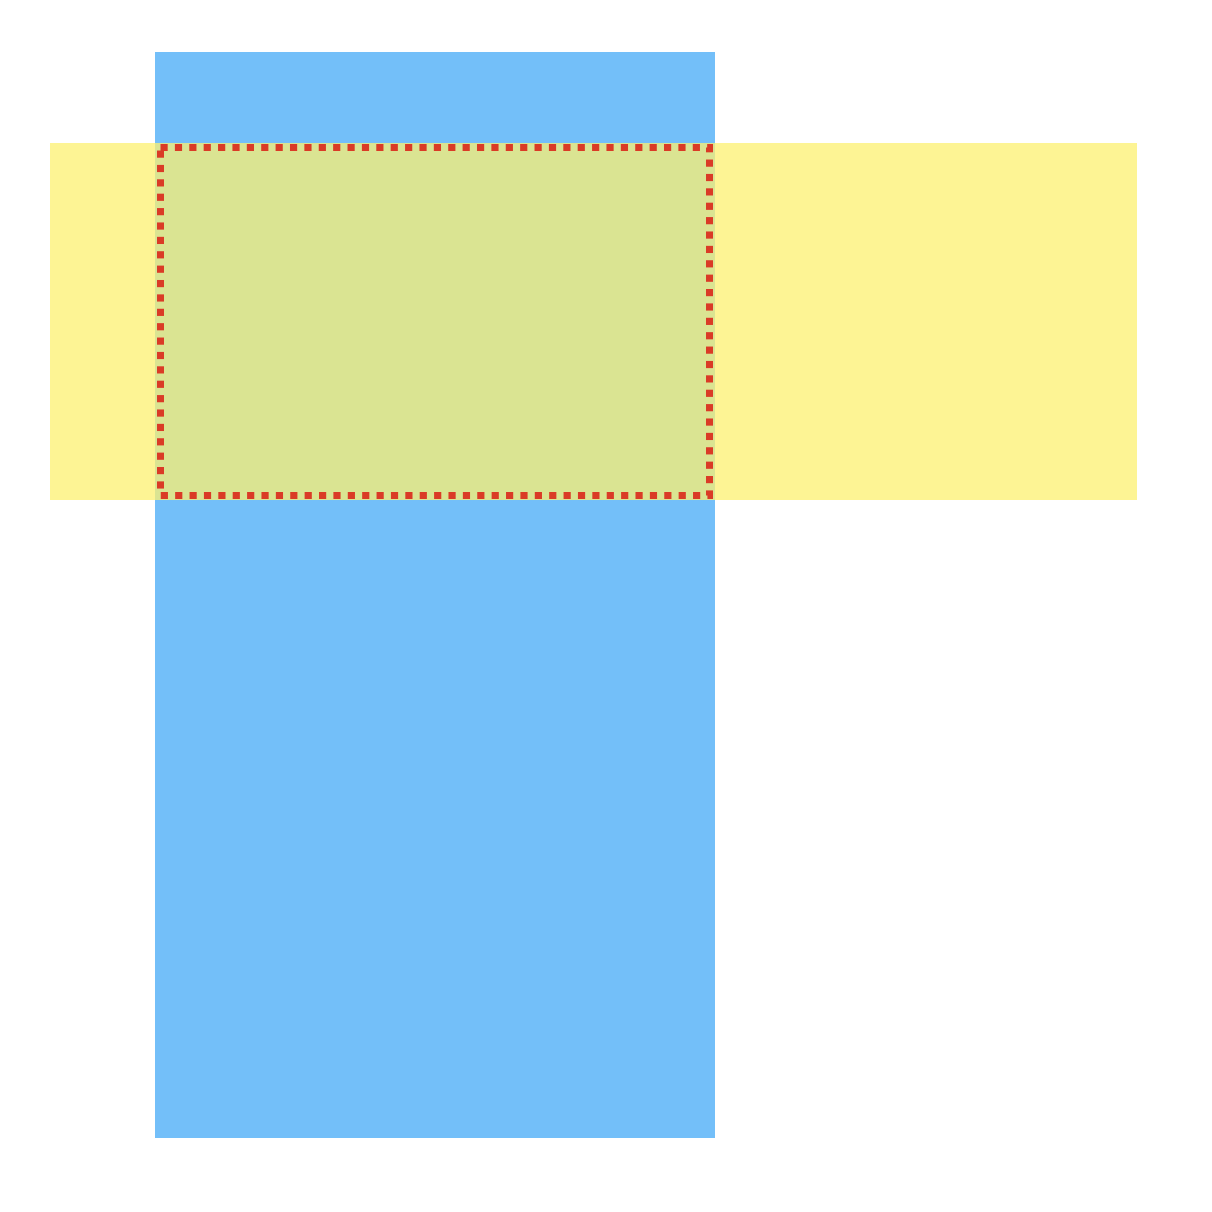
\includegraphics[width=\linewidth]{pics/scrollslider.png}
        \caption{ScrollSlider Funktionsweise}
        \label{fig:impl:scrollslider}
    \end{minipage}
    \hspace{.05\linewidth}
    \begin{minipage}[b]{.4\linewidth}
        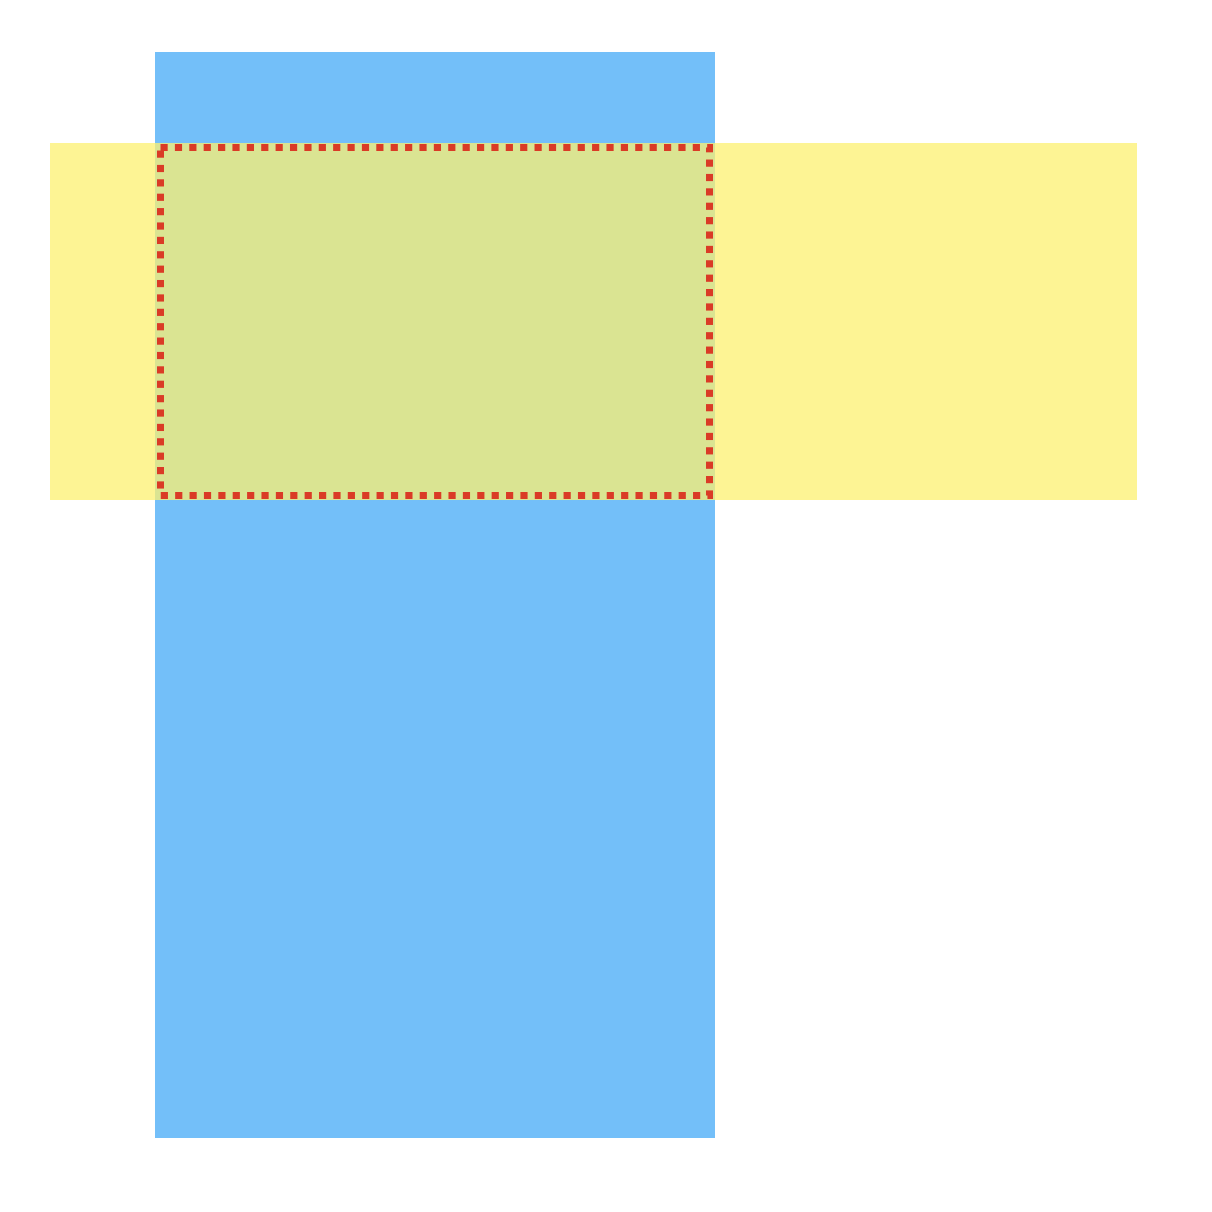
\includegraphics[width=\linewidth]{pics/scrollslider.png}
        \caption{ScrollSlider Funktionsweise}
        \label{fig:impl:scrollslider}
    \end{minipage}
 \end{figure}

Nach Implementierung dieses Tutorials wurde folgender Stand erreicht: Die blaue Box repräsentiert den typischen vertikalen Scrollverlauf auf der Webseite. Dieser Scrollwert wird dann prozentual auf die gelbe Box übertragen. Die gelbe Box wird somit um denselben Prozentwert nach links verschoben, wie der Benutzer nach unten scrollt. Dadurch bleibt für den Benutzer der Webseite immer nur der Bereich sichtbar, der sich innerhalb der rot gestrichelten Box befindet.

Diese Grundlage musste weiter bearbeitet werden, um dynamischen Inhalt zu akzeptieren, da bisher alle Breiten, die für die x-y-Transformation benötigt wurden, fest vorgegeben waren. Diese Berechnung reagiert auf das Laden der Seite, und die Breite bezieht sich auf das window-Objekt. Aus diesen Gründen ist eine dynamische Skalierung wie bei Media Queries in CSS nicht möglich. Wenn die Seitengröße verändert wird, muss die Seite neu geladen werden, damit sie korrekt dargestellt wird.

\subsubsection*{All Articles}

Eine weitere wichtige Komponentenrealisierung ist die All Articles Component. 

Die Funktion "All Articles" ermöglicht es, alle Artikel eines bestimmten Typs anzuzeigen, wofür innerhalb der Komponente eine eigene Fetch-Anfrage ausgeführt wird. Darüber hinaus bietet "All Articles" auch die Möglichkeit zur Filterung und zur Begrenzung der Seiten (beispielsweise 20 Artikel pro Seite, dann Seite 2).

\begin{figure}[H]
    \centering
    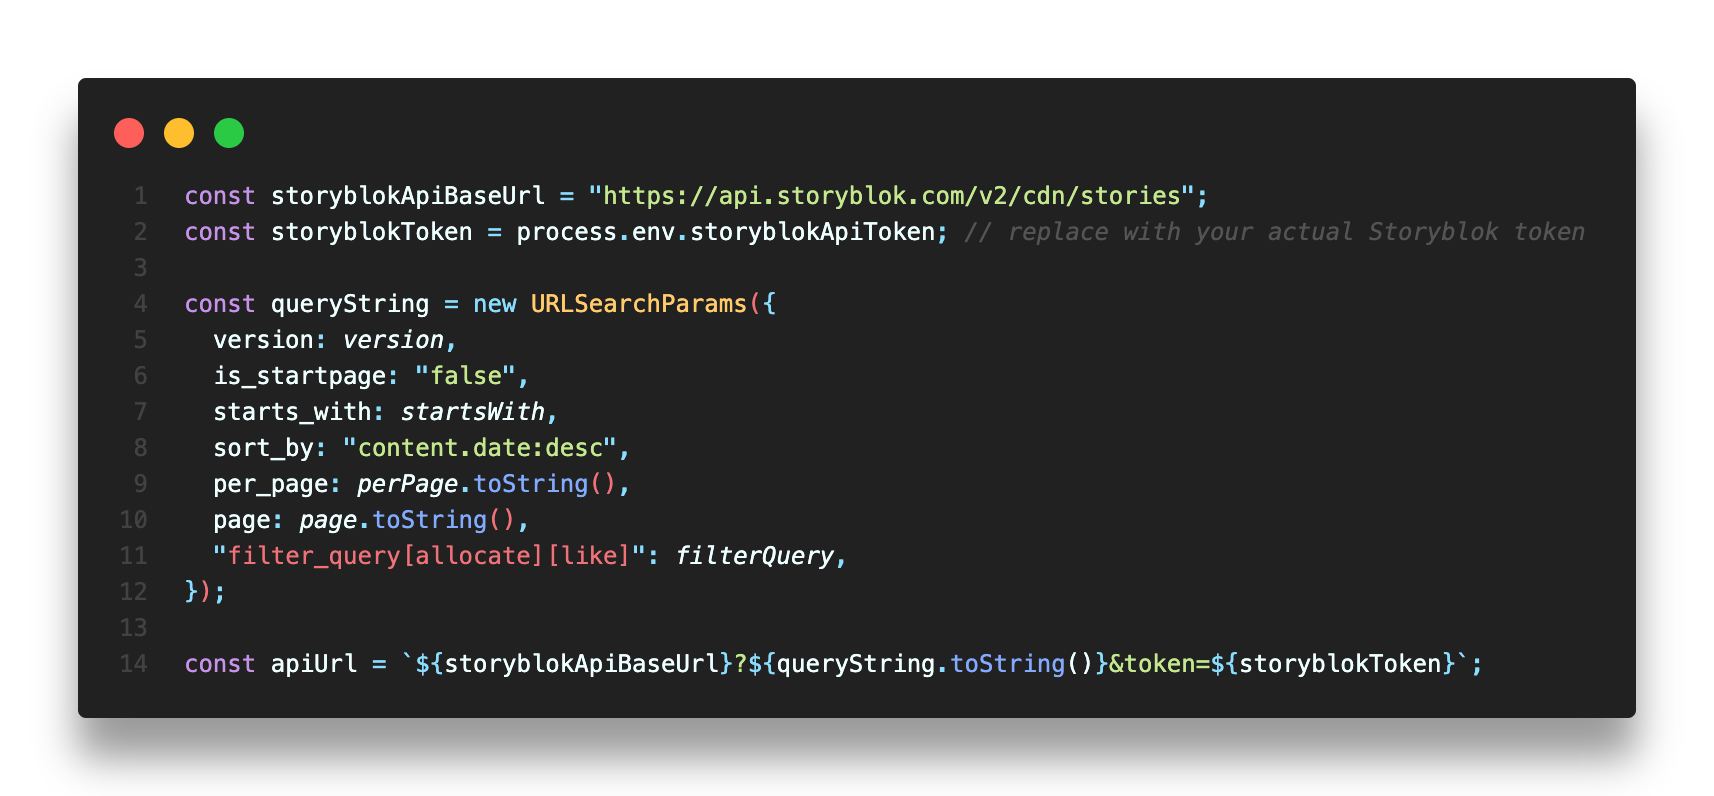
\includegraphics[width=\linewidth]{pics/allArticles.png}
    \caption{All Articles - Parameter}
    \label{fig:impl:allarticles:url}
\end{figure} 

\begin{figure}[H]
    \centering
    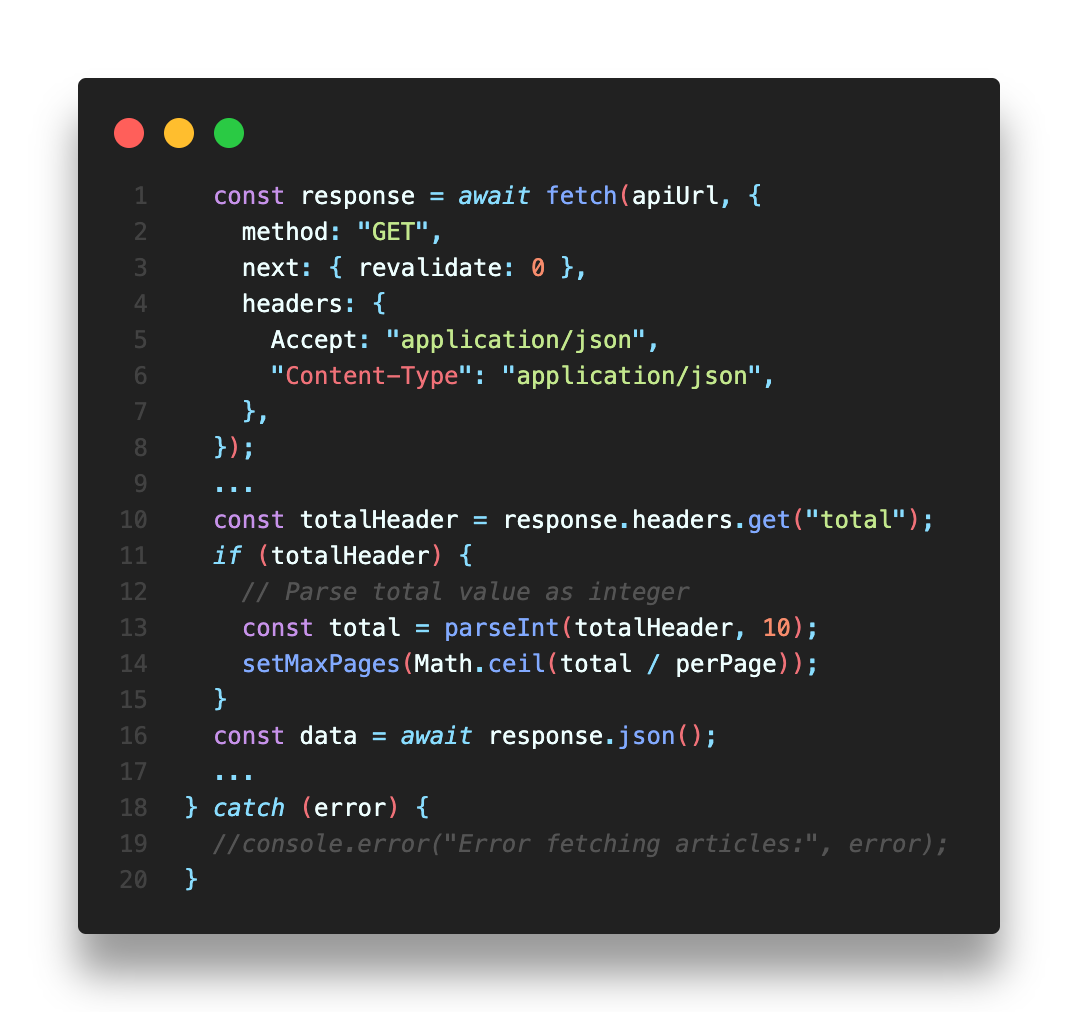
\includegraphics[width=\linewidth]{pics/allArticlesFetch.png}
    \caption{All Articles - Fetch}
    \label{fig:impl:allarticles:fetch}
\end{figure}

Um die richtigen Artikel zu erhalten, wird zunächst die Anfrage-URL zusammengestellt (siehe Abbildung \ref{fig:impl:allarticles:url}).

Anschließend wird im Antwort-Header der Wert total ausgelesen, um die maximale Seitenzahl berechnen zu können (siehe Abbildung \ref{fig:impl:allarticles:fetch}).

\subsubsection*{Hero}

Die Hero-Komponente bildet den obersten Teil der Webseite, ausgenommen der Startseite, auf der die Startanimation zu finden ist. Unser Hero zeichnet sich durch eine seitliche Schräge aus, die sich durch das gesamte Design der Webseite zieht. Auf diesem schrägen Banner, der sich ausschließlich rechts befindet, steht in großer weißer Schrift die Überschrift für die aufgerufene Seite. Als Hintergrund für den resultierenden Deltoiden wird ein thematisch passendes Bild verwendet.

\subsubsection*{ValueDokument ValueDokumentEntry}

Für die Darstellung der Werte der HTL wurden die Komponenten ValueDocument und ValueDocumentEntry erstellt. 
Eine große Herausforderung bestand darin, den Inhalt schräg zu positionieren oder den Text so zu platzieren, dass es den Anschein hat, als wäre er schräg platziert. 
Dies wurde wie folgt umgesetzt: Das Bild und der farbige Hintergrund wurden einfach per clip-path abgeschnitten. 
Der restliche Inhalt wurde durch dynamisches Margin so platziert, dass der Text nicht mehr abgeschnitten wird.

\subsubsection*{Timetable}

Um den Stundenplan der HTL anschaulich zu gestalten, wurde eine Timetable-Komponente entwickelt. 
Im Vollbildmodus wird ein virtueller Stundenplan angezeigt, der wie eine Kombination aus Stundenplänen aller fünf Jahre aussieht. 

\begin{figure}[H]
    \centering
    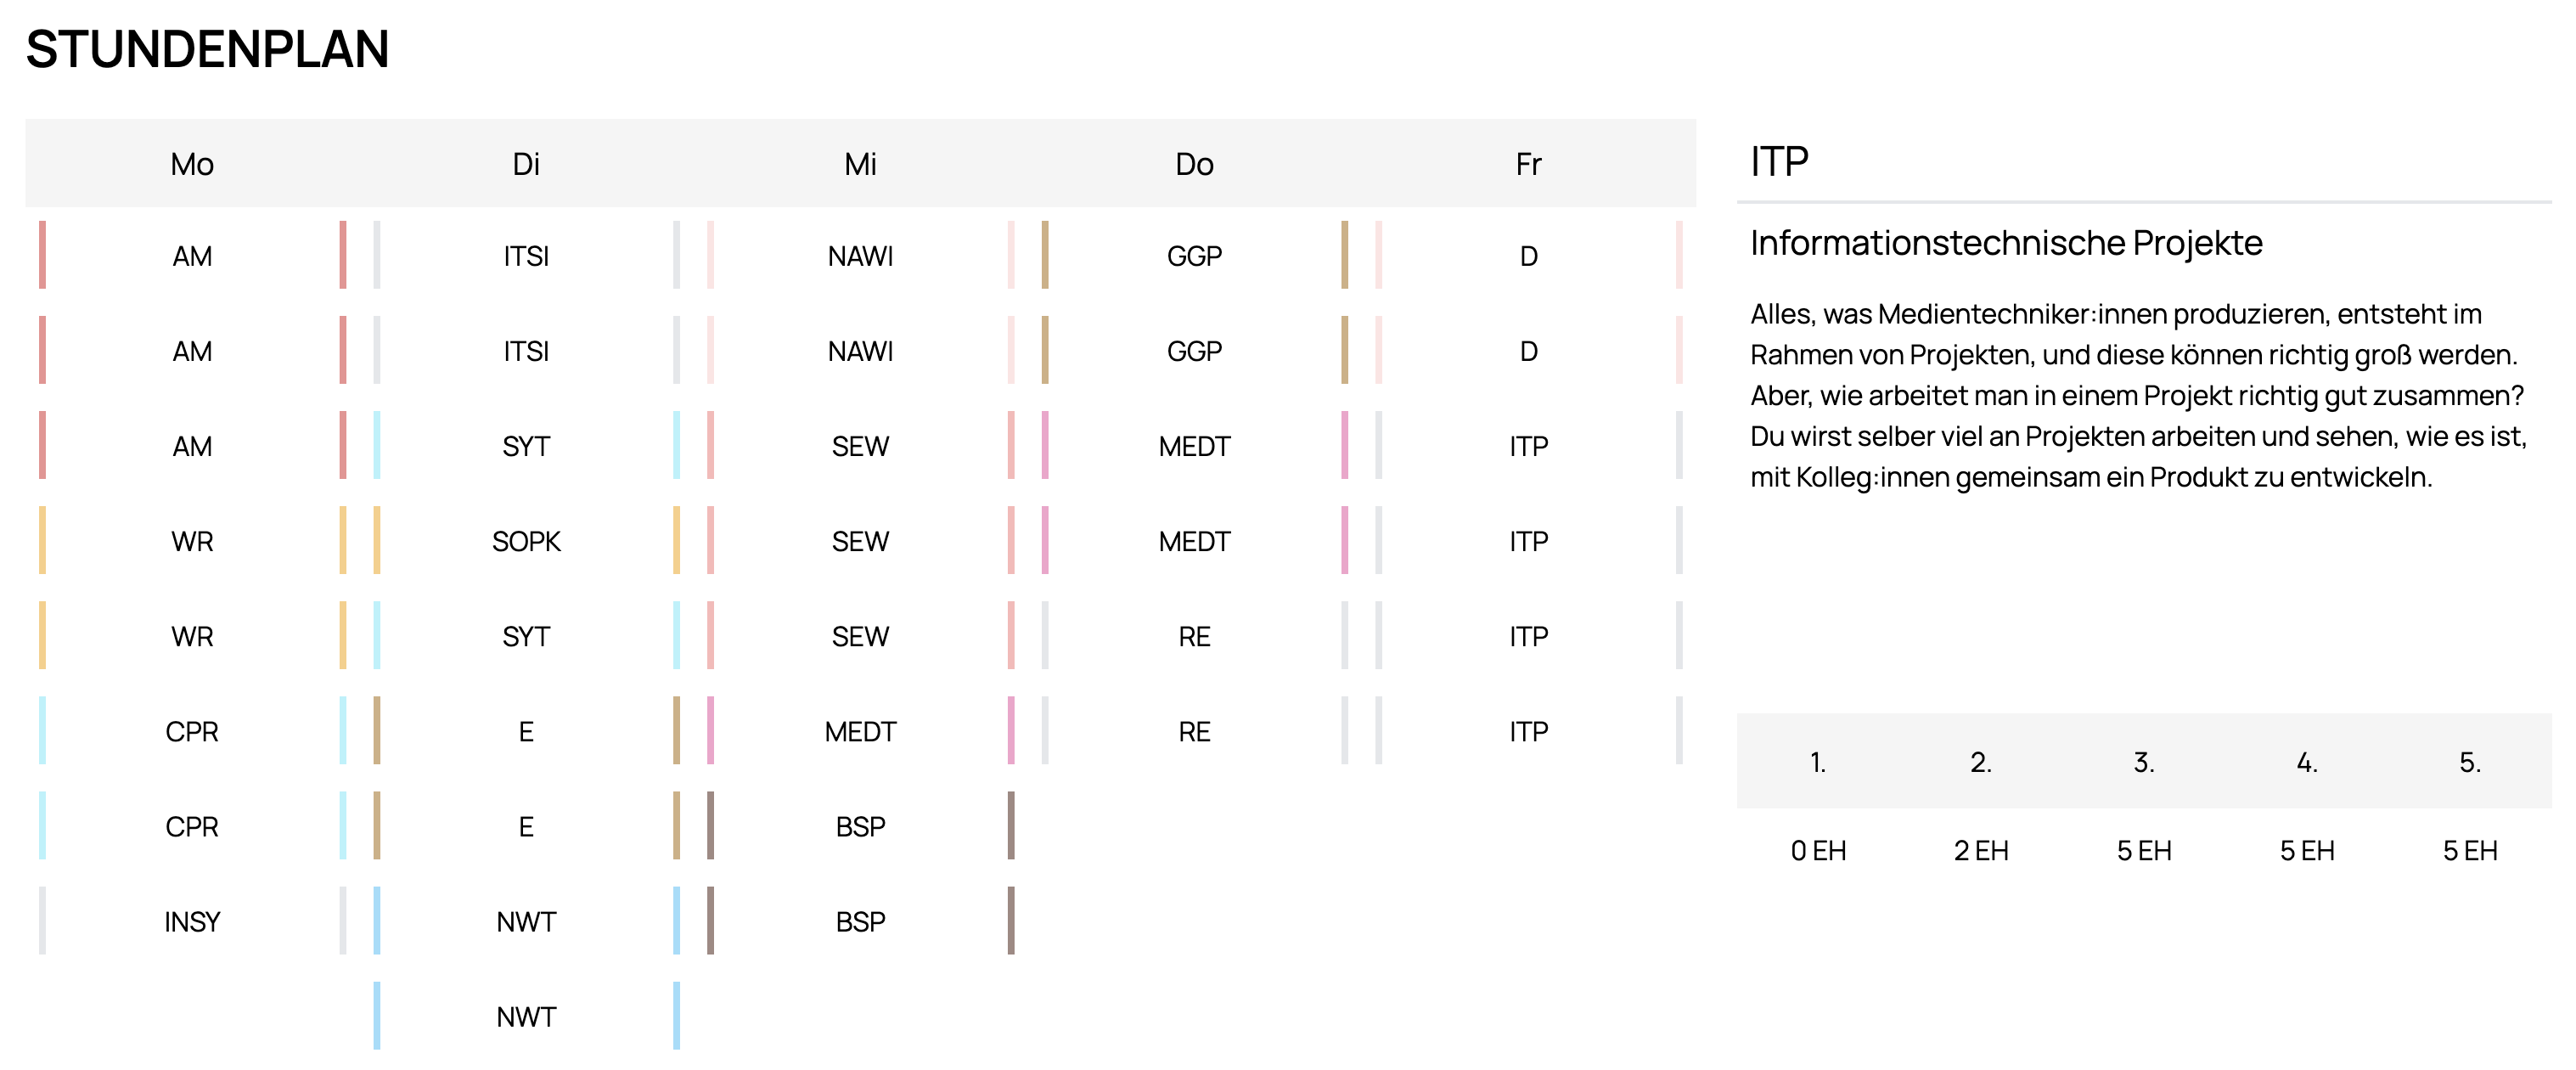
\includegraphics[width=\linewidth]{pics/timetable-big.png}
    \caption{Stundenplan und Beschreibung}
    \label{fig:impl:timetable}
\end{figure} 

Auf Mobilgeräten wird aufgrund des begrenzten Platzes eine zweispaltige Liste angezeigt. 
Dabei werden zunächst die Spezialfächer und anschließend die normalen Fächer aufgelistet. 
In beiden Designs werden die Farben der Fächer von WebUntis verwendet. 
Da die Abkürzung allein relativ wenig über das Fach aussagt, wurde zusätzlich ein Feld entwickelt, das nach dem Klicken auf das Fach weitere Informationen anzeigt (siehe Abbildung \ref{fig:impl:timetable} rechts).

\begin{figure}
    \begin{minipage}[b]{.4\linewidth} 
       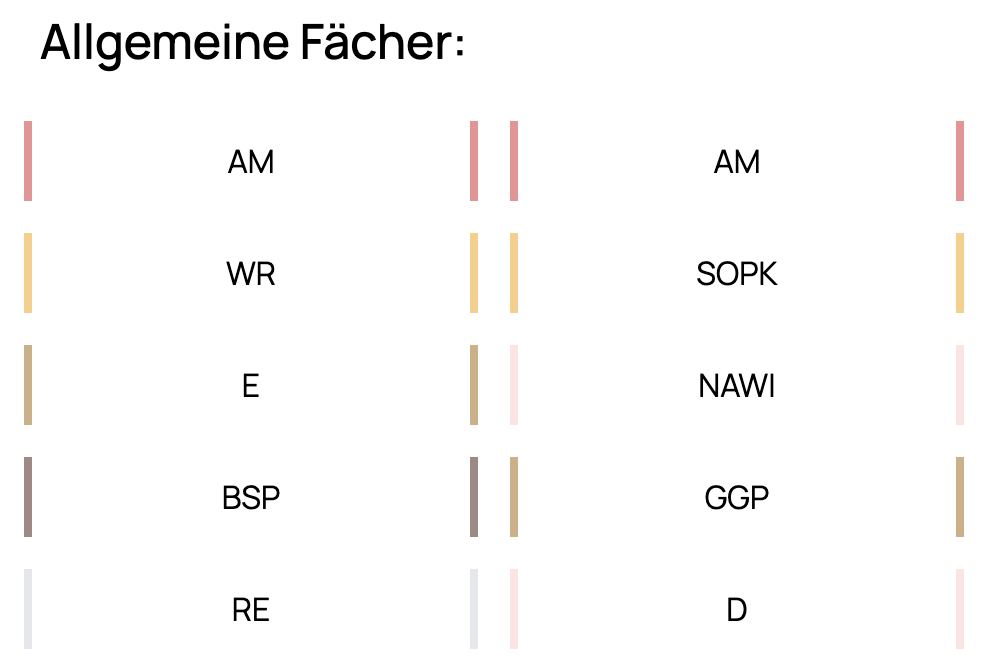
\includegraphics[width=\linewidth]{pics/timetable-allg.png}
       \caption{}
       \label{fig:impl:timetable_allg}
    \end{minipage}
    \hspace{.05\linewidth}
    \begin{minipage}[b]{.4\linewidth}
       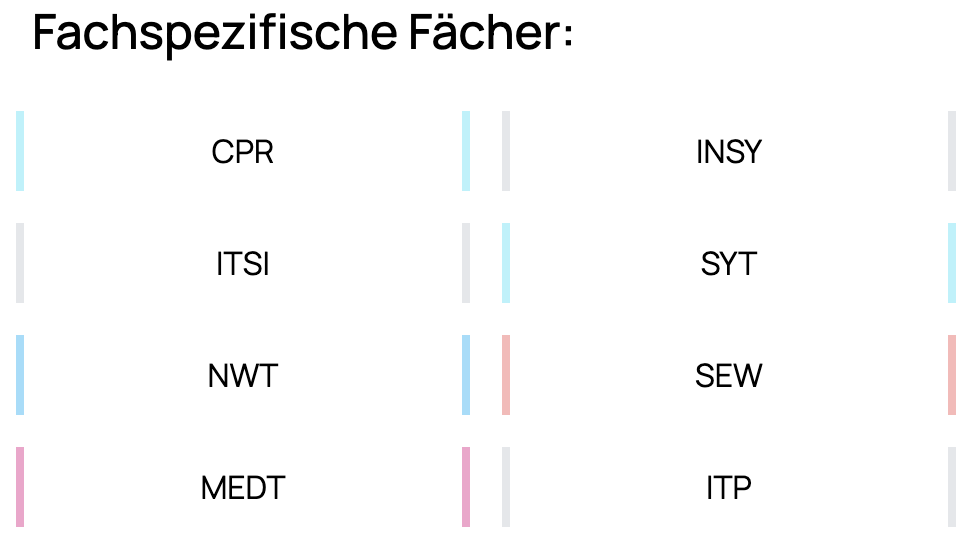
\includegraphics[width=\linewidth]{pics/timetable-spez.png}
       \caption{}
       \label{fig:impl:timetable_spez}
    \end{minipage}
 \end{figure}

\subsection{Internationalisierung}

Ein weiterer wichtiger Teil, der erst gegen Ende der Arbeit realisiert wurde, war die Internationalisierung. 
Hierbei stieß man jedoch auf Schwierigkeiten durch die Verwendung des neuen Next.js 13. 
Aufgrund der Nutzung dieses neuen Frameworks war es nicht mehr möglich, die automatische I18N Internationalisierung zu verwenden, weshalb man sie manuell implementieren musste. 
Unter Zuhilfenahme der offiziellen Next-Dokumentation, Stack Overflow und einigen Anpassungen an generiertem Code wurde dann die Middleware.js entwickelt, die die Internationalisierung handhabte.

Dies funktioniert, indem am Anfang der URL ein /de oder /en steht (Beispiel: www.htl-leonding.at/de). 
Wenn jedoch eine Seite ohne richtigen Sprachenparameter aufgerufen wird, passt die Middleware den Aufruf so an, dass die URL entsprechend dem aktuellen Standort des Endbenutzers die Sprache verwendet. 
Die ausgewählte Sprache ist außerdem wichtig, da sie für die Storyblok-Anfragen benötigt wird, damit die richtigen Daten angezeigt werden.

Da Flaggen zum Wechseln der Sprachen nicht in unser Design passen, wurde für den Wechsel ein einfacher illustrierter Globus mit einem zusätzlichen Code (DE für Deutsch und EN für Englisch) verwendet.

\subsection{Deployment}

Der letzte Teil der Arbeit beinhaltete das Deployment der erstellten Seite, um einen realen Betrieb zu simulieren. Dieser Vorgang wurde durch die Verwendung von Vercel und die Erstellung des Projekts in der CLI sowie der daraus resultierenden Ordnerstruktur sehr vereinfacht. In Vercel musste lediglich das GitHub-Repository verlinkt werden, und durch die unveränderte Ordnerstruktur wurde das Next.js 13 Projekt erkannt. Anschließend wurden nur noch die Schlüssel konfiguriert, die sonst in der .env Datei zu finden waren. Danach musste man nur noch kurz warten, und die Seite war auf Vercel gehostet. Ein Problem, das dabei auftrat, war, dass es nicht eindeutig im Fehler erkennbar war, wenn kein Schlüssel übergeben wurde. Des Weiteren wurden auch einige TypeScript-Probleme im Code aufgezeigt, die während der Entwicklung ignoriert worden waren. Nachdem diese Probleme jedoch schnell behoben wurden, war das Deployment inklusive der GitHub-Pipeline abgeschlossen.



